\documentclass[12pt]{article}
\usepackage[a4paper,margin=2.5cm]{geometry}
\usepackage[T1]{fontenc}
\usepackage[utf8]{inputenc}
\usepackage{lmodern}
\usepackage{microtype}
\usepackage{amsmath,amssymb}
\usepackage{booktabs}
\usepackage{graphicx}
\usepackage{eurosym}
\usepackage{setspace}
\usepackage[hidelinks]{hyperref}
\usepackage[round]{natbib}
\usepackage{caption}
\usepackage{pdflscape}
\usepackage{placeins}
\renewcommand{\topfraction}{0.9}\renewcommand{\bottomfraction}{0.9}\renewcommand{\textfraction}{0.05}\renewcommand{\floatpagefraction}{0.8}
\captionsetup{font=small,labelfont=bf}
\graphicspath{{figures/}}
\onehalfspacing

\title{Bunching at a Moving Threshold:\\ Firm Responses to Romania's Micro-Enterprise Tax, 2014--2025}
\author{Denis Siminiuc\thanks{Draft of \today. Data: Ministry of Finance, ANAF and ONRC open data via data.gov.ro. Replication package (pipeline, harmonised panel with hashed identifiers, legal timeline): \url{https://github.com/simdenis/romania-micro-enterprise-bunching}, data files on Zenodo, doi:10.5281/zenodo.22863290; it contains no names, birth dates or addresses. Drafting and code were produced with the assistance of a large language model (Anthropic Claude), including the initial text of every section and the analysis scripts; all analysis choices, the verification of legal references against primary sources and of numerical claims against the data, and the final text are the author's responsibility. Comments welcome.}}
\date{September 2026}

\begin{document}
\maketitle

\begin{abstract}
\noindent Romanian companies with revenue below a ceiling set in euro pay 1 to 3 percent of revenue in tax instead of 16 percent of profit. The ceiling moved six times between 2013 and 2026. Using the annual accounts of every company, 9.6 million firm-years, we show three things. First, reported revenue piles up just below the ceiling every year, the pile-up follows the ceiling when it moves, and within a fixed euro ceiling it sits within a few thousand lei of the ceiling's value at the previous year-end exchange rate and moves with that rate. Second, because the ceiling moved, each notch location can be compared with the same point of the distribution in years when no ceiling was there. This difference-in-bunching estimator needs no fitted curve. At 77 placebo locations it gives excess mass centred on zero with a standard deviation of 0.15; at every real notch it gives 2 to 8 percent of the firms within 20 percent of the ceiling, but only 0.06 to 0.30 percent of all firms. Bunching is large locally and trivial in aggregate; the regime's fiscal cost lies with the firms well below the ceiling. Third, the response comes from high-margin service firms, reported profit margins shift in the direction the tax incentive predicts when firms are moved between regimes, a 2023 rule requiring one employee doubled the rate at which zero-employee firms hired exactly one in the year it was enacted, and bunching is correlated with, but not shown to be caused by, the registration of sibling firms.
\end{abstract}

\section{Introduction}

Many countries tax small firms on their revenue and larger firms on their profit \citep{sharma2025dual, kanbur2014, dharmapala2011}. The size limit between the two regimes is a notch: crossing it switches the tax base from revenue to profit and, for a firm whose margin is above the ratio of the two rates, raises the tax bill at once. Firm responses to such notches have been measured at VAT thresholds in the United Kingdom \citep{liu2021vat}, Finland \citep{harju2019vat} and Spain \citep{almunia2018}, and at turnover-tax and corporate-tax cut-offs in Pakistan \citep{kleven2013}, Armenia \citep{asatryan2016}, South Africa \citep{boonzaaier2019} and Costa Rica \citep{bachas2021}. The choice between taxing revenue and taxing profit is itself the subject of \citet{best2015}, who show with Pakistan's minimum tax that a revenue base is harder to evade but distorts production; our setting switches the base for the same firms repeatedly. In most of these settings the limit rarely moves, so the distribution that would exist without the notch has to be extrapolated from the distribution away from it, usually with a polynomial. \citet{blomquist2021} show that this extrapolation is not identified without restrictions on the shape, and that the estimates depend on which restrictions one picks. \citet{best2018} compare the same location before and after a notch was introduced, and \citet{marx2024} uses panel variation.

Romania's limit moves. The micro-enterprise regime taxes revenue at 1 to 3 percent for companies whose annual revenue is below a ceiling set in euro, and the ceiling changed six times between 2013 and 2026: \euro{}65,000 until 2015, \euro{}100,000 in 2016, \euro{}500,000 in 2017, \euro{}1,000,000 from 2018 to 2022, \euro{}500,000 in 2023 and 2024, \euro{}250,000 in 2025 and \euro{}100,000 from 2026. Every location that was ever a notch was, in other years, an ordinary point of the revenue distribution. We use that variation to describe and to measure the response, and we use the side conditions that changed with the ceiling, an employee requirement and a rule on linked firms, to look at how firms respond.

The paper makes three points. First, the pile-up in reported revenue follows the ceiling up and down. Within a fixed euro ceiling it tracks the ceiling's lei value at the previous year-end exchange rate to within a few thousand lei a year. That settles the usual objection that firms simply report round numbers: a spike at 4,779,300 lei that moves to 4,869,400 lei the next year is not a rounding habit. When a future ceiling has been enacted, or announced and then withdrawn, a second spike appears at it. Second, the distribution at each notch location in years without a ceiling there serves as the counterfactual, under an assumption we state and test. At 77 placebo locations with no notch the estimator gives excess mass with mean 0.01, standard deviation 0.15 and a largest absolute value of 0.55. At each real notch it gives 2 to 8 percent of the firms within 20 percent of the ceiling, or 0.7 to 3.0 in the excess-mass statistic, with block-bootstrap standard errors of 0.07 to 0.16. In aggregate, though, the excess is 0.06 to 0.30 percent of all firms. Bunching is large next to the ceiling and small in the economy. The fiscal cost of the regime, and the policy debate about it \citep{ban2023, imf2025, cf2024}, concern the firms well below the ceiling, not the threshold. Third, the channels. Excess mass is two to three times higher in professional, administrative, health and information services than in trade and transport, and bunchers in those sectors report margins of 30 to 40 percent. When the 2018 increase in the ceiling moved firms onto the revenue tax, their reported margins rose by 0.7 points relative to firms left on profit tax; when the 2023 cut moved firms back, margins fell by 1 to 2 points. The regime changes what firms report, not only where they sit, as \citet{bachas2021} find for Costa Rica and as the revenue-base logic of \citet{best2015} predicts. A 2023 rule requiring at least one employee doubled the rate at which zero-employee firms hired exactly one in the year it was enacted. Firms at the ceiling are more likely to have a newly registered sibling firm, but the combined revenue of firms with the same administrator does not bunch, so we treat splitting as a correlation. Section~\ref{sec:margins} takes each channel in turn.

Section~\ref{sec:inst} describes the regime, Section~\ref{sec:data} the data, Section~\ref{sec:method} the estimator, Section~\ref{sec:results} the main results and Section~\ref{sec:margins} the channels. Section~\ref{sec:conc} concludes.

\FloatBarrier
\section{Institutional background}\label{sec:inst}

The micro-enterprise income tax (\emph{impozitul pe veniturile microîntreprinderilor}), Title III of the Fiscal Code (Law 227/2015) and before 2016 Title IV$^1$ of Law 571/2003, replaces the 16 percent profit tax with a tax on revenue for companies that meet a set of conditions. The main condition is that revenue in the previous fiscal year was below a ceiling set in euro. Table~\ref{tab:thresholds} gives the ceiling and rates and Table~\ref{tab:conditions} the side conditions by year of revenue; Appendix~\ref{app:legal} gives the acts.

\begin{table}[!tbp]\centering\small
\caption{Micro-enterprise regime: ceiling and rates by year of revenue}\label{tab:thresholds}
\begin{tabular}{lll}\toprule
Revenue year & Ceiling (EUR) & Rate on revenue \\ \midrule
2013--2015 & 65,000 & 3\% \\
2016 & 100,000 & 1\% ($\ge$ 2 employees), 2\% (1), 3\% (none) \\
2017 & 500,000 (from 1 Feb.) & 1\% ($\ge$ 1 employee), 3\% (none) \\
2018--2022 & 1,000,000 & 1\% ($\ge$ 1 employee), 3\% (none) \\
2023 & 500,000 & 1\% \\
2024 & 500,000 & 1\% up to \euro{}60,000; 3\% above or in listed activities \\
2025 & 250,000 & 1\% up to \euro{}60,000; 3\% above or in listed activities \\
2026 & 100,000 & 1\% \\ \bottomrule
\end{tabular}
\end{table}

\begin{table}[!tbp]\centering\small
\caption{Micro-enterprise regime: side conditions by year of revenue}\label{tab:conditions}
\begin{tabular}{p{2.2cm}p{12.5cm}}\toprule
Years & Conditions \\ \midrule
2013--2015 & Mandatory (opt-out for new firms with capital $\ge$ \euro{}25,000). Consulting and management revenue at most 20\% (from 2014). Exceeding the ceiling in-year re-taxed the whole year. \\
2016--2017 & Mandatory, opt-out for capital $\ge$ 45,000 lei (from 2017). In-year exit from the quarter of crossing. Consulting cap retained. \\
2018--2022 & Mandatory, opt-out for capital $\ge$ 45,000 lei with two employees (from April 2018). Consulting cap abolished. \\
2023 & Optional; exit permanent. At least one employee. Consulting cap 20\%. A person holding over 25\% may be a shareholder in at most three micro-enterprises. Hospitality firms exempt from the ceiling. \\
2024 & At most one micro-enterprise per person holding over 25\%. Ceiling tested on linked enterprises combined. Consulting cap reformulated. \\
2025 & Consulting cap abolished. Status for 2026 tested on 2025 revenue against \euro{}100,000. \\
2026 & Base changed to accounting turnover including linked enterprises. \\ \bottomrule
\end{tabular}
\end{table}

Three features matter for what follows. The first is timing. Under the in-year rule, a micro-enterprise whose cumulated revenue passes the ceiling during year $t$ owes profit tax from that quarter (for 2013 to 2015, for the whole year). The ceiling is converted at the central bank (BNR) rate at the close of year $t-1$. Under the year-end rule, status for year $t+1$ depends on revenue at 31 December of year $t$, converted at the rate at the close of year $t$. When the ceiling is unchanged the two rules put the notch a few thousand lei apart, and in a depreciating currency the in-year rule, which uses the earlier and lower rate, is the one that binds. When a cut has been enacted for the following year, a firm faces two notches at once. That happened in 2022: Ordinance 16/2022 of July 2022 set \euro{}500,000 for 2023 status based on 2022 revenue, and Law 370/2022 of 20 December 2022 then deferred the revenue test to 2023 revenue while keeping the employee and ownership conditions at 31 December 2022. It happened again in 2025, when Ordinance 156/2024 of 31 December 2024 set \euro{}250,000 for 2025 and \euro{}100,000 for 2026 status based on 2025 revenue.

The second feature is the tax base. The ceiling is tested on the taxable base of Article 53, which leaves out a short list of items such as subsidies, provision reversals and, from 2021, dividends received. The accounts report total revenue, which is the same or larger. For most small firms the excluded items are zero; where they are not, the firm looks closer to the ceiling than it is, which shifts the bunching region slightly to the right in our data. From 2026 the base is accounting turnover.

The third is the set of side conditions in Table~\ref{tab:conditions}. The employee condition is met by a full-time contract, by part-time contracts adding up to a full-time position, or by a paid mandate contract. Linked enterprises are defined by holdings above 25 percent. The activities taxed at 3 percent regardless of revenue in 2024 and 2025 are software, hospitality, legal and medical services. The 20 percent cap on consulting and management revenue, in force in 2014--2017 and 2023, is a margin the accounts do not let us see.

The VAT exemption for small firms is a separate notch, on turnover as defined in Article 310(2) and set in lei: 220,000 lei until March 2018, 300,000 lei from 1 April 2018 (Law 72/2018) and 395,000 lei from 1 September 2025 (Ordinance 22/2025). In 2024 the lei value of the \euro{}60,000 rate boundary is within 1,500 lei of 300,000, so the two cannot be told apart; in 2025 the VAT threshold moved away and the boundary can be seen on its own (Section~\ref{sec:vat}).

\FloatBarrier
\section{Data}\label{sec:data}

\paragraph{Financial statements.} The Ministry of Finance publishes, for each fiscal year, the main figures from the annual accounts of every company, identified by its fiscal code (CUI) and CAEN activity code: balance-sheet totals, net turnover, total revenue, total expenses, gross and net profit or loss, and average headcount. There are two forms, the micro-entity form and the full form. Their layout is stable from 2016; the 2014 and 2015 files use an older set of columns, which we harmonise. The 2021, 2023 and 2025 files were published a few weeks after the filing deadline, the others are later re-issues, so late filers are covered unevenly; about 40,000 small firms appear in 2020 and 2022 but not in 2021. Table~\ref{tab:panel} summarises the panel: 9.58 million firm-years after removing 32 duplicate records, 1.56 million firms. Total revenue is the variable for the micro-enterprise notch; net turnover is the variable for the VAT threshold.

\begin{table}[!tbp]\centering
\small
\caption{Statement panel, 2014--2025}\label{tab:panel}
\resizebox{\linewidth}{!}{%
\begin{tabular}{lrrrr}\toprule
Year & Firm-years & Revenue $>0$ & Median revenue (k lei) & EUR/RON, 31 Dec \\ \midrule
2014 & 676,868 & 495,914 & 124 & 4.4821 \\
2015 & 681,821 & 505,212 & 141 & 4.5245 \\
2016 & 700,249 & 526,282 & 146 & 4.5411 \\
2017 & 732,051 & 553,283 & 151 & 4.6597 \\
2018 & 757,929 & 579,309 & 162 & 4.6639 \\
2019 & 792,376 & 616,900 & 173 & 4.7793 \\
2020 & 815,779 & 636,361 & 162 & 4.8694 \\
2021 & 781,470 & 624,795 & 188 & 4.9481 \\
2022 & 862,564 & 693,309 & 207 & 4.9474 \\
2023 & 890,836 & 716,718 & 223 & 4.9746 \\
2024 & 968,594 & 769,620 & 226 & 4.9741 \\
2025 & 918,232 & 738,762 & 239 & 5.0985 \\
\bottomrule\end{tabular}}
\begin{minipage}{0.95\linewidth}\vspace{2pt}\footnotesize Source: Ministry of Finance annual financial statements (micro-entity and full forms) via data.gov.ro; BNR year-end reference rate. Median revenue is over firms with positive revenue. 32 duplicated firm-years (30 in 2016) removed; about 600 firm-years per year with negative revenue are excluded from all windows.\end{minipage}
\end{table}

\paragraph{Tax regime.} The accounts do not say which regime a firm is in. We recover it in two ways. First, gross profit minus net profit is the income tax accrued. Divided by revenue it is roughly 1, 2 or 3 percent for micro-enterprises; divided by pre-tax profit it is roughly 16 percent for profit-tax firms. The gap also contains the specific tax on hospitality firms in 2017--2022 and other taxes on the result, net of sponsorship and cash-register credits, so ratios such as 0.8 or 2.4 percent occur, and a firm with positive tax and a pre-tax loss is most likely, but not certainly, a micro-enterprise. Second, the ANAF taxpayer registry, a snapshot dated 31 August 2023, has one column per tax a firm is registered for; in its column dictionary, obligation 120 is the micro-enterprise income tax and obligation 100 the profit tax. Table~\ref{tab:crosscheck} cross-tabulates the two measures for 2023. Of firms registered for the micro-enterprise tax, 84 percent show a micro-enterprise tax pattern and 1 percent a profit-tax pattern. Of firms registered for profit tax, 22 percent show the profit-tax pattern, 8 percent a micro pattern, and half paid no tax, which is what loss-making and dormant profit-tax firms look like. Where both measures are decisive, 57 percent of firms, they agree in 92.5 percent of cases; 2.6 percent of 2023 filers are not in the registry. The inference picks out micro-enterprises well and profit-tax firms poorly, so we use the registry flag where regime membership matters and the accounts-based measure only as a check.

\begin{table}[tbp]\centering
\small
\caption{Tax regime inferred from the 2023 statements versus the ANAF tax-vector flag (June 2023)}\label{tab:crosscheck}
\resizebox{\linewidth}{!}{%
\begin{tabular}{lrrrr}\toprule
Regime inferred from statements & ANAF: micro & ANAF: profit & ANAF: other/none & Not in ANAF \\ \midrule
Micro (tax $\approx$ 1--3\% of revenue) & 277,265 & 19,677 & 312 & 7,102 \\
Micro (tax $>0$, pre-tax loss) & 103,544 & 14,248 & 87 & 1,966 \\
Profit tax ($\approx$ 16\% of profit) & 4,421 & 92,503 & 64 & 2,045 \\
No tax paid & 34,486 & 220,021 & 273 & 10,942 \\
Ambiguous & 16,047 & 30,596 & 60 & 437 \\
Other & 19,272 & 34,966 & 158 & 344 \\
\bottomrule\end{tabular}}
\begin{minipage}{0.95\linewidth}\vspace{2pt}\footnotesize ANAF flags: IMP120 = registered for micro-enterprise income tax, IMP100 = registered for profit tax. Where both measures are decisive, they agree for 92.5\% of firms.\end{minipage}
\end{table}

\paragraph{Employees.} Average headcount is blank for a quarter of small firms and reported as zero for a further 5 percent. We treat blanks as zero. Among micro-enterprises in 2017 to 2022, when the 3 percent rate applied to firms without employees, three quarters of blank-headcount firms paid the 3 percent rate, which supports the choice. The field is a whole number in every record and behaves like a flag for having had an employee at some point in the year, not a time-weighted average: of firms that go from zero to one employee in 2022, 12 percent paid the no-employee rate for most of that year, which a true average would have rounded to zero. Late-year hires are therefore counted, and the 2022 timing below is real. The legal test is met by a full-time contract, by part-time contracts adding up to one, or by a paid mandate contract, and the field distinguishes none of these, so headcount is a proxy in both directions.

\paragraph{Trade register.} The National Trade Register Office publishes snapshots of all registered firms, with registration date, legal form and address, and a table of legal representatives with name, date and place of birth. We use the snapshot of 2 September 2026, key persons on name, birth date and birth place, hash the key, and keep administrators and legal representatives. The register lists administrators as of the snapshot date, not shareholders and not past administrators, so common administration is our proxy for common ownership. The open data has a representatives table only in snapshots from November 2025 onwards, so administrators at the time of the 2018--2023 observations cannot be recovered, and a firm whose administrator changed since is mismeasured. Eighty-five percent of the limited-liability companies in the sample have exactly one administrator, for whom the proxy is close; company names carry no usable marker of sole ownership. Nearly all filers, 96 to 99 percent by year, link to at least one administrator, and the linked share is the same across the groups compared below. Four percent of administrator records lack a birth date, so their key is the name alone; results are reported with and without them. Names, birth dates and addresses are used only to build hashed keys and appear in no output or replication file.

\paragraph{Exchange rates.} BNR reference rates at the last quotation of each year.

\FloatBarrier
\section{Empirical strategy}\label{sec:method}

For each year $t$ the notch location is $L_t = T_t \, e_{t-1}$, where $T_t$ is the euro ceiling for revenue in year $t$ and $e_{t-1}$ the BNR rate at the close of year $t-1$. Let $F_t$ be the distribution of revenue in year $t$ and $q_t = F_t(L_t)$ the quantile of the notch. For every other year $c$, let $L^*_c = F_c^{-1}(q_t)$ be the revenue at the same quantile. Year $c$ is an admissible control if no known notch of year $c$, the micro ceiling, an enacted or announced future ceiling, the \euro{}60,000 rate boundary, or the VAT threshold, lies within 25 percent of $L^*_c$. Bins are 1 percent of the notch location wide, in a window of $\pm$20 percent, and shares $s_{t,k}$ are bin counts divided by the count in the window. The counterfactual share is the mean of $s_{c,k}$ over admissible controls. Excess mass is
\begin{equation}
b_t = \frac{\sum_{k \in B} \left( s_{t,k} - \bar{s}_{c,k} \right)}{\frac{1}{|B|}\sum_{k\in B} \bar{s}_{c,k}},
\end{equation}
where $B$ is the five bins just below the notch. The missing mass $m_t$ is the same sum over the five bins just above, negative when the treated density falls short of the control there. The identifying assumption is that the shape of the revenue density around a given quantile is the same across years, apart from the notch. Matching on quantiles makes the counterfactual immune to inflation and to growth in firm size, but not to changes in the shape of the distribution. Because shares are normalised within the window, the excess and the missing mass must offset within it, so $m_t$ is not independent evidence. We report a multinomial bootstrap, a block bootstrap that resamples control years, and, as the most relevant measure of uncertainty, the distribution of $b$ at 77 placebo locations, at 0.45 to 2.5 times each year's ceiling and themselves at least 25 percent from any notch. Since $b$ is per bin it scales with bin width; with 1 percent bins $b$ is roughly the width of the bunching region in percent of the ceiling. We also report the excess number of firms below the notch, which does not depend on bin width, its range over regions of 3, 5 and 8 percent, and the excess as a share of all filers in the year, $B/N_t$. The admissibility rule is applied to the matched location rather than the window edges, so a control window can include the region above another year's notch; this affects only bins above the notch. Appendix Table~\ref{tab:controls} lists, for every notch and control year, the matched revenue and its distance to the nearest notch that year, so the rule can be checked; the closest admissible cases are 26 to 34 percent away, all for the 2014--2016 notches against the VAT thresholds. Tightening the rule to 35 percent leaves every estimate from 2017 on unchanged, moves the 2014 estimate from 1.15 to 1.07 and the 2016 estimate from 1.56 to 1.55, and leaves 2015 with no admissible control year.

\FloatBarrier
\section{Results}\label{sec:results}

\subsection{The spike tracks the exchange rate}

From 2018 to 2022 the euro ceiling stayed at \euro{}1,000,000, but its lei value rose from 4.66 to 4.95 million lei as the leu depreciated. Figure~\ref{fig:lei} shows the revenue distribution in lei with 10,000-lei bins. The spike moves with the ceiling each year. Table~\ref{tab:lei} locates the modal 5,000-lei bin: in every year it is 1,400 to 5,600 lei below the ceiling at the previous year-end rate, while the ceiling at the current year-end rate is 80,000 to 115,000 lei further right in 2019 to 2021. Firms target the in-year rule, which is also the lower of the two lei values, so the two explanations coincide. Nobody rounds revenue to 4,779,300 lei; a spike at that value that moves to 4,869,400 lei the next year is not round-number reporting or an accounting convention.

\begin{figure}[!tbp]\centering
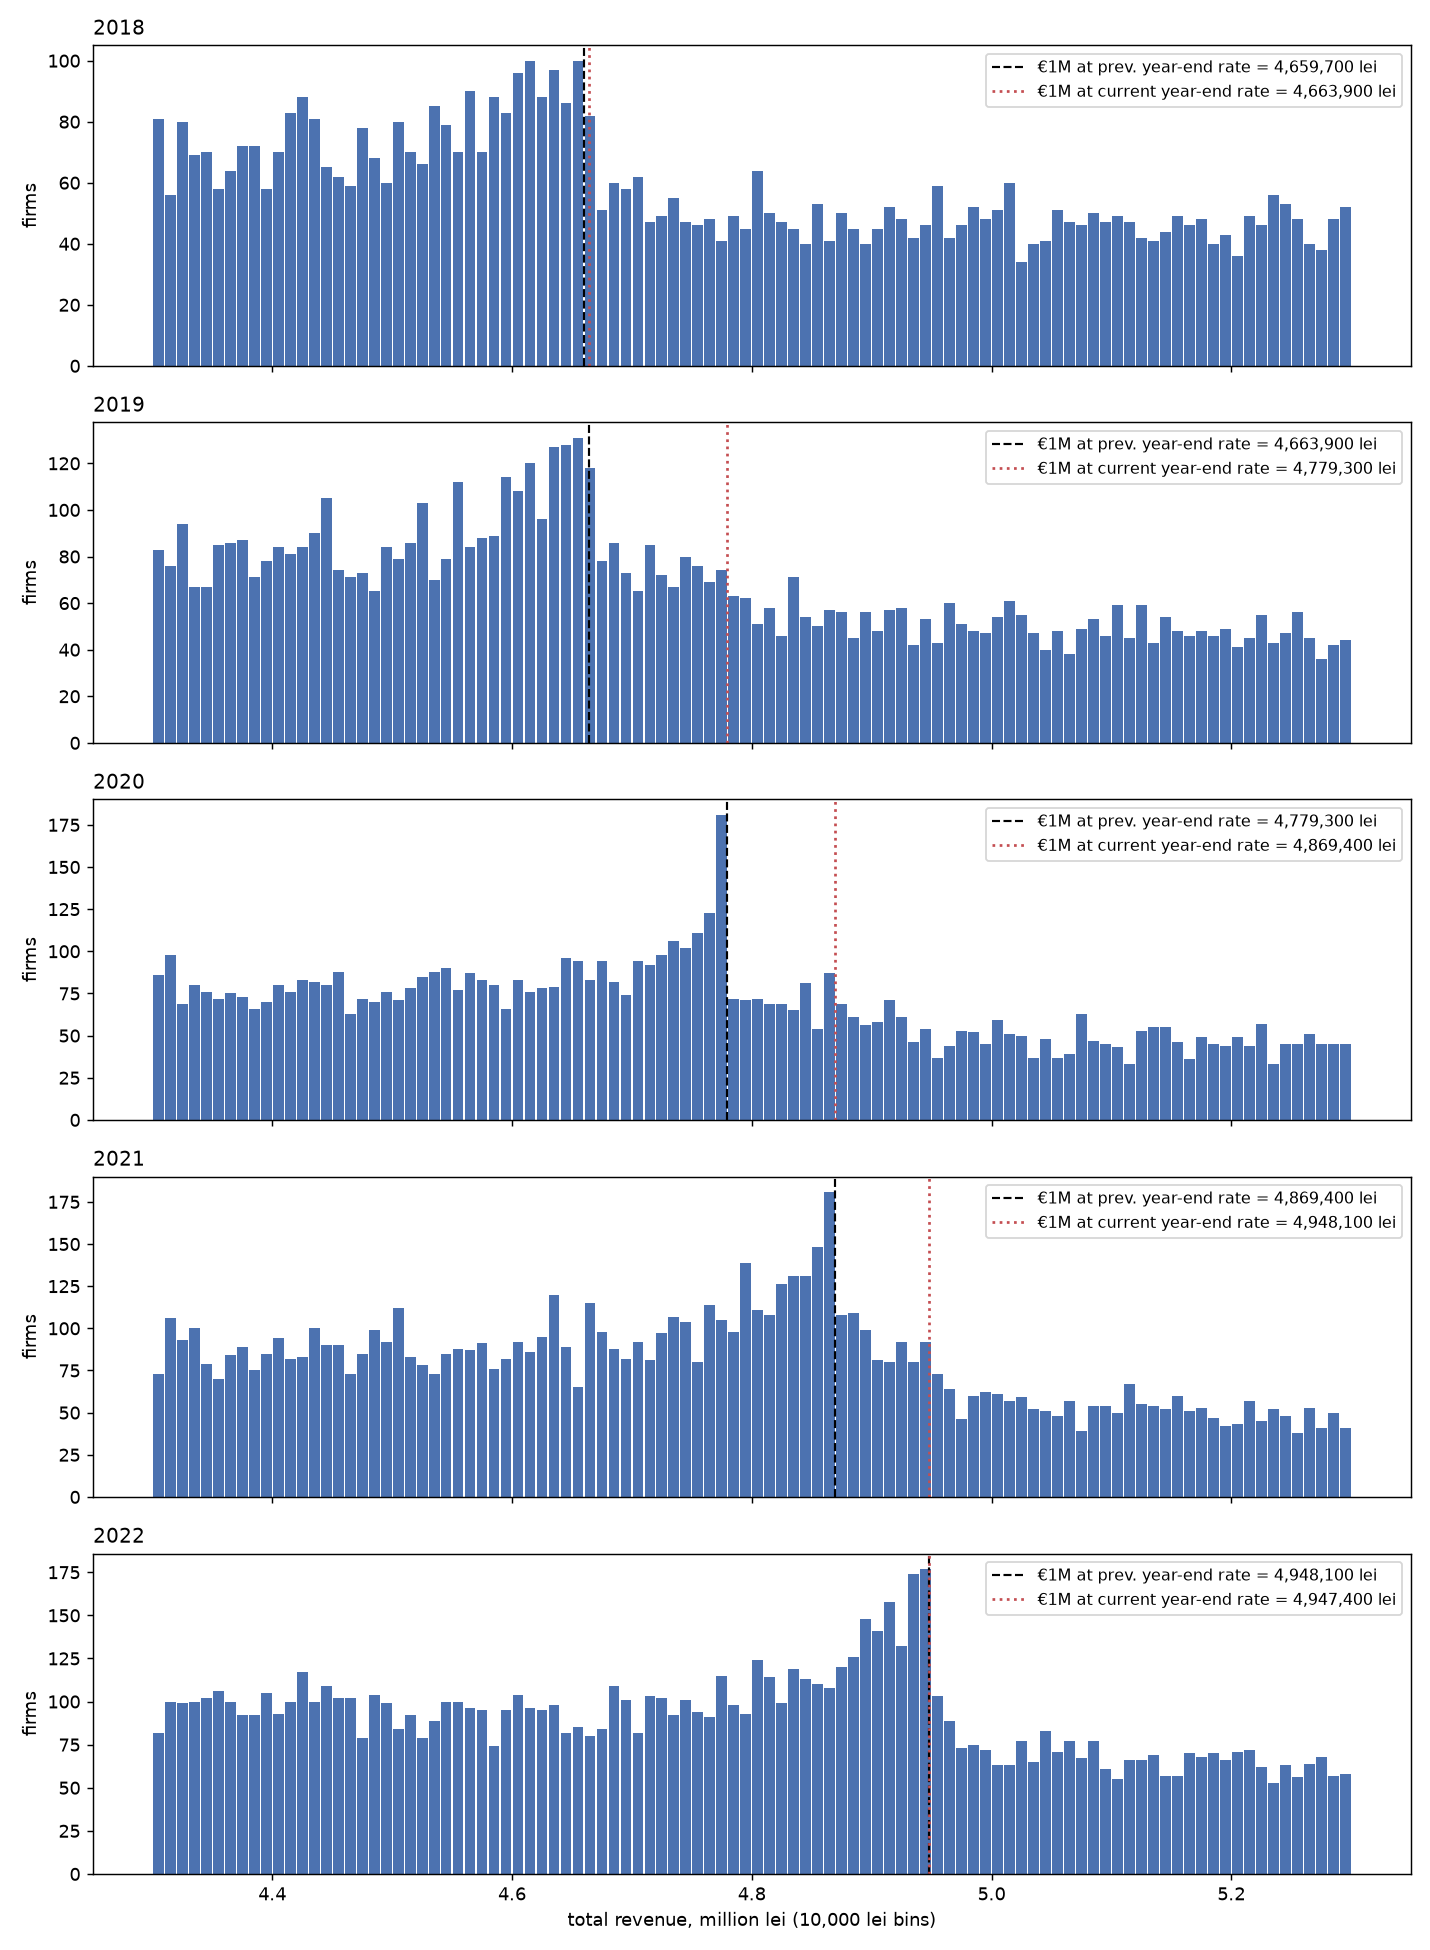
\includegraphics[width=0.85\textwidth]{lei_tracking_1M_2018_2022.png}
\caption{Total revenue in lei around \euro{}1,000,000, 2018--2022, 10,000-lei bins. Dashed: ceiling at the previous year-end rate; dotted: at the current year-end rate.}\label{fig:lei}
\end{figure}

\begin{landscape}
\begin{table}[htbp]\centering
\small
\caption{Location of the revenue spike in lei, 2018--2022}\label{tab:lei}
\resizebox{\linewidth}{!}{%
\begin{tabular}{lrrlrrr}\toprule
Year & \euro{}1M at prev.\ year-end rate & \euro{}1M at current year-end rate & Modal 5,000-lei bin & Firms in it & Bin centre minus prev.-rate threshold & Current minus prev.-rate threshold \\ \midrule
2018 & 4,659,700 & 4,663,900 & 4,655,000-4,660,000 & 59 & -2,200 & +4,200 \\
2019 & 4,663,900 & 4,779,300 & 4,660,000-4,665,000 & 73 & -1,400 & +115,400 \\
2020 & 4,779,300 & 4,869,400 & 4,775,000-4,780,000 & 95 & -1,800 & +90,100 \\
2021 & 4,869,400 & 4,948,100 & 4,865,000-4,870,000 & 105 & -1,900 & +78,700 \\
2022 & 4,948,100 & 4,947,400 & 4,940,000-4,945,000 & 101 & -5,600 & -700 \\
\bottomrule\end{tabular}}
\begin{minipage}{0.95\linewidth}\vspace{2pt}\footnotesize Modal 5,000-lei bin within 60,000 lei of either candidate threshold. At 1,000-lei resolution the modal bins hold only 16 to 31 firms and are noisier; they lie 2,000 to 5,000 lei below the previous-rate threshold in 2020--2022 and further below in 2018--2019.\end{minipage}
\end{table}
\end{landscape}

\subsection{The spike follows the ceiling}

Figure~\ref{fig:panels} shows a spike in the bin just below the ceiling in every year. It is at \euro{}65,000 in 2014 and 2015, moves to \euro{}100,000 in 2016 and \euro{}500,000 in 2017, stays at \euro{}1,000,000 from 2018 to 2022, returns to \euro{}500,000 in 2023 and 2024 and moves to \euro{}250,000 in 2025. In 2014 and 2015 a second, taller spike is visible at about \euro{}49,000, which is 220,000 lei, the VAT threshold of the time. In 2014 the spike straddles the computed notch rather than sitting below it, consistent with the whole-year re-taxation rule then in force and with the base issue noted above.

\begin{figure}[!tbp]\centering

\includegraphics[width=\textwidth]{bunching_panels.png}
\caption{Total revenue around the micro-enterprise ceiling, 2014--2025, converted at the BNR rate at the close of the previous year. Dashed: ceiling; dotted: ceiling at the current year-end rate. In the 2014 and 2015 panels the red line is a polynomial counterfactual of degree 5 excluding three bins on each side, shown to make the point that it passes through the VAT spike, which lies inside its fitting window.}\label{fig:panels}
\end{figure}

\subsection{Difference-in-bunching estimates}

Table~\ref{tab:dib} reports the estimates and Figure~\ref{fig:dib} the densities for four notches; Appendix Figure~\ref{fig:dibfull} shows all fourteen. In every year the treated density exceeds the same-quantile control density in the bins just below the notch, and the control density is smooth through it. Excess mass in the 5 percent region below the notch ranges from 1.9 percent of firms in the window, at the \euro{}500,000 ceiling of 2017 and the \euro{}250,000 ceiling of 2025, to 7.6 percent at the \euro{}500,000 ceiling of 2023. At the 77 placebo locations $b$ has mean 0.01, standard deviation 0.15 and a largest absolute value of 0.55. Every notch estimate exceeds the largest placebo, most by a factor of two or more; the 2017 and 2025 in-year estimates, 0.76 and 0.73, are only one and a half placebo standard deviations above it and are the weakest in the set. Two things dilute the 2025 notch: the enacted \euro{}100,000 ceiling for 2026 competed for the same firms' attention, and at the 3 percent rate that applied above \euro{}60,000 the break-even margin is 18.75 percent, above the 13.5 percent median margin of that year's bunchers, so crossing raised taxes for fewer firms.

As a share of all filers, the excess is 0.06 to 0.30 percent of firms (Table~\ref{tab:robust}). This is the number to carry into the policy discussion. The response at the threshold is large next to it and negligible in the economy: the revenue at stake in the regime comes from the hundreds of thousands of firms taxed at 1 to 3 percent of revenue well below the ceiling, not from the few thousand that keep their revenue under it. Table~\ref{tab:robust} shows that a block bootstrap over control years gives standard errors of 0.07 to 0.16, in line with the placebo spread; that dropping any one control year moves $b$ by less than 0.1; and that narrowing the window lowers $b$ and widening it raises it, because the normalisation is within the window, while the excess counts are unchanged. Appendix Table~\ref{tab:robustextra} adds that correcting the control quantile for the bunchers themselves changes $b$ by at most 0.1, that control years before and after the treated year give similar estimates, and that keeping only firms present in the adjacent years lowers $b$ by 0.05 to 0.2.

Three patterns stand out. First, excess mass at the \euro{}1,000,000 ceiling grows from 3.5 percent of the window in 2018 to 5.5 percent in 2021, in line with the gradual build-up of bunching found by \citet{kleven2013}. Second, 2023 is the largest response, at 7.6 percent, falling to 4.1 percent in 2024 at the same ceiling. Two things changed in 2023: the ceiling halved, so many firms sat at the new notch, and exit from the regime became permanent, so crossing cost more. One might think firms pushed above the new ceiling pulled revenue back down to requalify, and 29.6 percent of the 2023 bunchers had indeed been above \euro{}500,000 in 2022. But the same is true at that location in years when it was not a threshold, because firms just below any point tend to be firms that were above it the year before. The ratio to a comparison group further below is 1.78 in 2023 against 1.55 to 1.96 in placebo years (Appendix Table~\ref{tab:transition}), so the inflow from above is mean reversion. Third, the two extra rows show a second notch at work. In 2022 the ceiling in force was \euro{}1,000,000, but from July to December 2022 firms expected 2023 status to depend on 2022 revenue being below \euro{}500,000. A spike of 2.0 percent of the window appears there, with none at that location in 2021; the December deferral came too late to undo it. In 2025 the same happens at \euro{}100,000, enacted in December 2024 for 2026 status: 3.7 percent of the window in excess, at the lei value of \euro{}100,000 at the end-2024 rate, the last rate firms could see, rather than at the end-2025 rate the law prescribes. The modal 1,000-lei bin is 496,000 to 497,000 lei against 497,410 lei for \euro{}100,000 at the end-2024 rate; a round-number spike would sit at 499,000 to 500,000, and does not.

For comparison, a polynomial counterfactual of the kind used by \citet{chetty2011} gives excess-mass estimates of 0.4 to 2.0 in a baseline specification, and across 27 combinations of bin width, polynomial degree and excluded window they range from negative values to more than twice the baseline in most years, even at a fixed bin width, which is the concern raised by \citet{blomquist2021}. The difference-in-bunching estimates fit no curve, and the placebo distribution is the honest measure of their uncertainty.

\begin{table}[htbp]\centering
\footnotesize
\caption{Difference-in-bunching estimates}\label{tab:dib}
\resizebox{\linewidth}{!}{%
\begin{tabular}{llrrrrrr}\toprule
Notch & Location (M lei) & Firms in window & $b$ (SE) & $m$ & Excess firms & \% of window & Range 3--8\% \\ \midrule
2014: in-year, \euro{}65,000 & 0.292 & 33,859 & 1.15 (0.08) & 0.77 & 986 & 2.9 & 932--931 \\
2015: in-year, \euro{}65,000 & 0.291 & 34,896 & 1.71 (0.09) & -0.39 & 1,526 & 4.4 & 1,232--1,674 \\
2016: in-year, \euro{}100,000 & 0.452 & 32,891 & 1.56 (0.08) & -0.25 & 1,321 & 4.0 & 985--1,493 \\
2017: in-year, \euro{}500,000 & 2.271 & 17,172 & 0.76 (0.11) & -0.26 & 332 & 1.9 & 262--370 \\
2018: in-year, \euro{}1,000,000 & 4.660 & 11,424 & 1.41 (0.14) & -0.59 & 406 & 3.5 & 341--467 \\
2019: in-year, \euro{}1,000,000 & 4.664 & 13,105 & 1.67 (0.13) & 0.05 & 558 & 4.3 & 494--605 \\
2020: in-year, \euro{}1,000,000 & 4.779 & 12,693 & 1.75 (0.14) & -0.01 & 576 & 4.5 & 473--655 \\
2021: in-year, \euro{}1,000,000 & 4.869 & 14,394 & 2.15 (0.13) & -0.08 & 793 & 5.5 & 670--916 \\
2022: in-year, \euro{}1,000,000 & 4.948 & 16,448 & 1.92 (0.13) & -0.45 & 808 & 4.9 & 711--829 \\
2023: in-year, \euro{}500,000 & 2.474 & 28,379 & 2.99 (0.11) & -0.14 & 2,151 & 7.6 & 1,850--2,388 \\
2024: in-year, \euro{}500,000 & 2.487 & 28,619 & 1.62 (0.10) & -0.28 & 1,179 & 4.1 & 945--1,339 \\
2025: in-year, \euro{}250,000 & 1.244 & 37,048 & 0.73 (0.08) & -0.06 & 690 & 1.9 & 588--697 \\
2022: announced, \euro{}500,000 & 2.474 & 24,241 & 0.80 (0.10) & -0.13 & 494 & 2.0 & 359--531 \\
2025: year-end, \euro{}100,000 & 0.497 & 55,232 & 1.47 (0.07) & 0.47 & 2,059 & 3.7 & 1,616--2,278 \\
\bottomrule\end{tabular}}
\begin{minipage}{0.95\linewidth}\vspace{2pt}\footnotesize Location = EUR threshold $\times$ BNR rate at the close of the previous year (in-year notches; the 2025 year-end notch at the end-2024 rate). Window $\pm$20\%, bins 1\% of the location. Control years are listed in Appendix Table~\ref{tab:controls}. $b$ = excess mass in the five bins below the notch in units of counterfactual firms per bin; $m$ = the same over the five bins above, negative meaning a deficit (a hole) and positive an excess; SE from 300 multinomial bootstrap draws. Excess firms = excess in the 5\% region below the notch, with its range over 3\% and 8\% regions.\end{minipage}
\end{table}
\begin{landscape}
\begin{table}[htbp]\centering
\footnotesize
\caption{Robustness of the difference-in-bunching estimates}\label{tab:robust}
\resizebox{\linewidth}{!}{%
\begin{tabular}{lrrrrrrrrrr}\toprule
Notch & $b$ & block-boot.\ SE & quantile-corr. & window $\pm$10\% & $\pm$30\% & pre only & post only & leave-one-out & continuing & $B/N_t$ (\%) \\ \midrule
2014: in-year, \euro{}65,000 & 1.15 & 0.08 & 1.14 & 0.74 & 0.78 & -- & 1.15 & 1.13--1.18 & 1.15 & 0.20 \\
2015: in-year, \euro{}65,000 & 1.71 & 0.08 & 1.70 & 1.36 & 1.55 & -- & 1.71 & 1.69--1.72 & 1.71 & 0.30 \\
2016: in-year, \euro{}100,000 & 1.56 & 0.11 & 1.56 & 1.23 & 1.70 & 1.30 & 1.63 & 1.54--1.64 & 1.45 & 0.25 \\
2017: in-year, \euro{}500,000 & 0.76 & 0.12 & 0.77 & 0.62 & 0.79 & 0.62 & 0.85 & 0.73--0.79 & 0.72 & 0.06 \\
2018: in-year, \euro{}1,000,000 & 1.41 & 0.14 & 1.36 & 1.20 & 1.46 & 1.44 & 1.37 & 1.38--1.43 & 1.35 & 0.07 \\
2019: in-year, \euro{}1,000,000 & 1.67 & 0.14 & 1.75 & 1.27 & 1.87 & 1.64 & 1.70 & 1.63--1.71 & 1.58 & 0.09 \\
2020: in-year, \euro{}1,000,000 & 1.75 & 0.16 & 1.87 & 1.35 & 1.93 & 1.64 & 1.90 & 1.71--1.83 & 1.67 & 0.09 \\
2021: in-year, \euro{}1,000,000 & 2.15 & 0.15 & 2.19 & 1.59 & 2.39 & 2.23 & 2.04 & 2.10--2.20 & 2.08 & 0.13 \\
2022: in-year, \euro{}1,000,000 & 1.92 & 0.14 & 1.97 & 1.58 & 2.15 & 1.82 & 2.05 & 1.87--1.97 & 1.77 & 0.12 \\
2023: in-year, \euro{}500,000 & 2.99 & 0.11 & 2.99 & 2.19 & 3.35 & 3.02 & 2.82 & 2.97--3.02 & 2.80 & 0.30 \\
2024: in-year, \euro{}500,000 & 1.62 & 0.09 & 1.65 & 1.26 & 1.78 & 1.64 & 1.52 & 1.58--1.64 & 1.58 & 0.15 \\
2025: in-year, \euro{}250,000 & 0.73 & 0.08 & 0.72 & 0.57 & 0.78 & 0.73 & -- & 0.71--0.75 & 0.61 & 0.09 \\
2022: announced, \euro{}500,000 & 0.80 & 0.10 & 0.79 & 0.60 & 0.89 & 0.80 & 0.83 & 0.78--0.82 & 0.83 & 0.07 \\
2025: year-end, \euro{}100,000 & 1.47 & 0.07 & 1.47 & 1.02 & 1.11 & 1.47 & -- & 1.44--1.50 & 1.43 & 0.28 \\
\bottomrule\end{tabular}}
\begin{minipage}{0.95\linewidth}\vspace{2pt}\footnotesize Baseline: window $\pm$20\%, all admissible control years. Block-bootstrap SE: control years resampled with replacement and treated bin counts resampled, 500 draws. Quantile-corrected: control quantile shifted down by $B/N_t$. Pre/post: only control years before/after the treated year. Leave-one-out: range of $b$ dropping one control year at a time. Continuing: firms with positive revenue in $t-1$, $t$ and $t+1$. $B/N_t$: excess firms in the 5\% region as a share of all filers with positive revenue in year $t$.\end{minipage}
\end{table}
\end{landscape}

\begin{figure}[!tbp]\centering
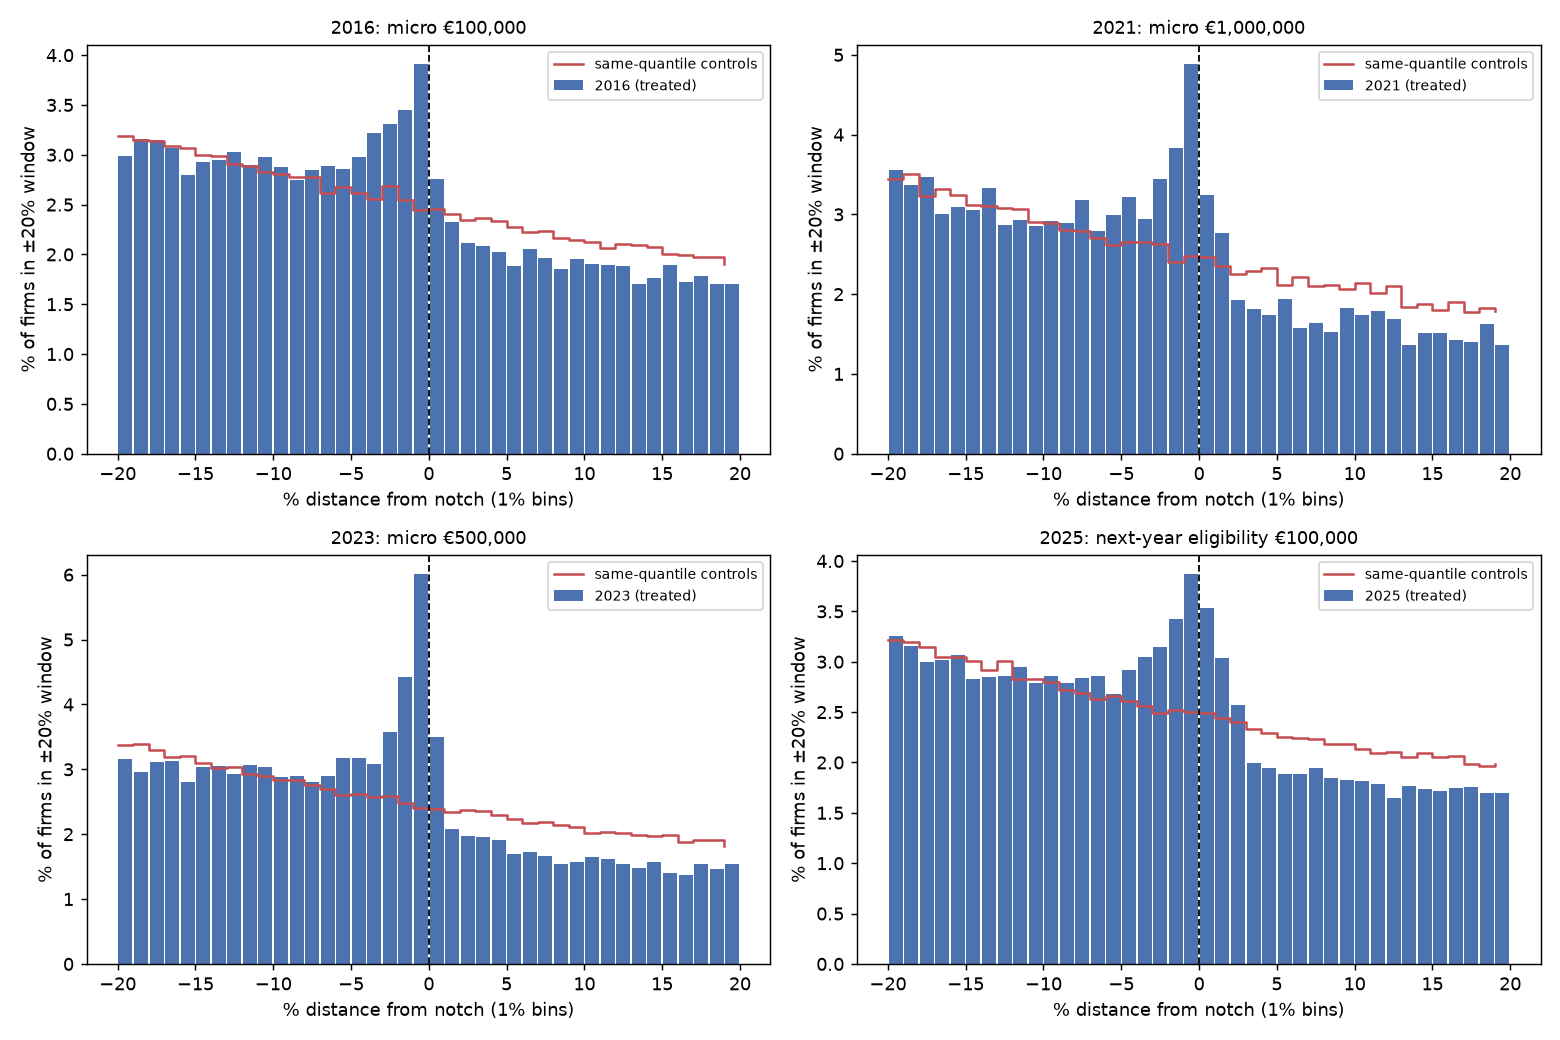
\includegraphics[width=\textwidth]{diff_in_bunching_4panel.png}
\caption{Treated-year density (bars) and same-quantile control density (line) around four notches, bins of 1 percent of the notch location. All fourteen notches in Appendix Figure~\ref{fig:dibfull}.}\label{fig:dib}
\end{figure}

\FloatBarrier
\subsection{Who bunches: margins and sectors}

The notch raises taxes only for firms whose margin exceeds the ratio of the two rates: 6.25 percent at a 1 percent revenue tax and 18.75 percent at 3 percent. Table~\ref{tab:margins} shows that firms in the 5 percent below the ceiling report median pre-tax margins of 11 to 20 percent, against 6 to 10 percent for firms just above and 7 to 12 percent for firms further below. Table~\ref{tab:sector} shows where they are. In 2023, excess mass is 12 to 15 percent of the window in professional, administrative, health and real-estate services and 10 percent in information and communication, against 5 percent in trade, 3.5 percent in transport and 1 percent in agriculture. Bunchers in the service sectors report margins of 29 to 43 percent, against 10 to 12 percent in trade and transport. The same ordering holds at the \euro{}250,000 ceiling of 2025, where information services lead at 5 percent and trade shows none. The sectors that bunch are the ones the 2023--2024 reforms singled out, and the ones where the regime saves the most tax per leu of revenue.

\begin{table}[!tbp]\centering
\small
\caption{Pre-tax profit margin by position relative to the threshold}\label{tab:margins}
\resizebox{\linewidth}{!}{%
\begin{tabular}{lrrrrr}\toprule
Year & Bunchers (0--5\% below) & Just above (0--10\%) & 10--25\% below & Bunchers: margin $>$ 6.25\% (\%) & Just above: margin $>$ 6.25\% (\%) \\ \midrule
2018 & 0.106 & 0.057 & 0.074 & 62 & 47 \\
2019 & 0.117 & 0.070 & 0.090 & 65 & 53 \\
2020 & 0.132 & 0.078 & 0.094 & 69 & 56 \\
2021 & 0.160 & 0.097 & 0.122 & 74 & 63 \\
2022 & 0.166 & 0.101 & 0.117 & 75 & 63 \\
2023 & 0.200 & 0.098 & 0.124 & 76 & 60 \\
2024 & 0.151 & 0.081 & 0.099 & 68 & 56 \\
2025 & 0.135 & 0.093 & 0.101 & 64 & 58 \\
\bottomrule\end{tabular}}
\begin{minipage}{0.95\linewidth}\vspace{2pt}\footnotesize Median of pre-tax profit over total revenue. At a 1\% turnover tax and a 16\% profit tax, the regime lowers the tax bill only for firms with margins above 6.25\%; at 3\% the break-even margin is 18.75\%.\end{minipage}
\end{table}
\begin{table}[htbp]\centering
\small
\caption{Excess mass by sector, in percent of firms within 20\% of the notch}\label{tab:sector}
\resizebox{\linewidth}{!}{%
\begin{tabular}{lrrrrr}\toprule
CAEN section & 2021 (\euro{}1M) & 2023 (\euro{}500k) & 2025 (\euro{}250k) & Firms in 2023 window & Median margin of 2023 bunchers \\ \midrule
Professional services & -- & 14.8 & 4.6 & 2,068 & 0.39 \\
Administrative services & -- & 13.3 & 3.4 & 1,089 & 0.29 \\
Construction & 7.4 & 12.6 & 3.1 & 4,078 & 0.25 \\
Health & -- & 12.0 & 2.6 & 896 & 0.32 \\
Real estate & -- & 11.2 & 3.5 & 908 & 0.43 \\
Information and communication & -- & 10.1 & 5.1 & 1,124 & 0.34 \\
Manufacturing & 2.9 & 6.5 & 1.9 & 3,008 & 0.16 \\
Trade & 5.3 & 4.8 & 0.3 & 8,426 & 0.12 \\
Transport & 6.1 & 3.5 & -0.2 & 2,428 & 0.10 \\
Agriculture & 0.5 & 1.0 & 1.0 & 1,653 & 0.08 \\
Hospitality & -- & 0.9 & 0.4 & 1,571 & 0.14 \\
Arts, other services & -- & -- & 1.7 & -- & -- \\
\bottomrule\end{tabular}}
\begin{minipage}{0.95\linewidth}\vspace{2pt}\footnotesize Difference-in-bunching within each CAEN section, matched at the section's own quantile, same control years as the pooled estimate; sections with fewer than 800 firms in the window omitted. Hospitality faced no revenue ceiling in 2023.\end{minipage}
\end{table}
\FloatBarrier

\subsection{Reported margins respond to the regime}

Reported margins are not neutral to the regime. A micro-enterprise's tax does not depend on its profit, a profit-tax firm's does, so firms on profit tax have a reason to report low margins that micro-enterprises lack. The ceiling changes let us test this. In 2018 the ceiling rose from \euro{}500,000 to \euro{}1,000,000, so every firm with 2017 revenue between those values was moved from profit tax to revenue tax without doing anything, while firms above \euro{}1,000,000 stayed on profit tax; in 2023 the cut reversed the move. Wide bands, (\euro{}500,000, \euro{}1,000,000] against (\euro{}1,000,000, \euro{}2,000,000], compare firms that differ twofold in size and produce mean-reversion drift of up to 1.5 points in a placebo design (Appendix Table~\ref{tab:eventstudy}). That motivates the narrowed bands of Table~\ref{tab:eventnarrow}: 20 percent either side of the cut-off, assigned on two-year average revenue, with placebos built at the same time, the same bands at cut-offs of \euro{}1,500,000 and \euro{}2,000,000 in the same base years, where no regime changed. With narrow bands the raw pre-period differences are within 0.2 points of zero and the contemporaneous placebos are within 0.5 points of zero before and after, so the correction is small and creates no pre-trend. Entry into the revenue-tax regime in 2018 raises the treated group's median margin by 0.7 points in the first year (standard error 0.2), from a base of about 6 percent; net of the placebos, 0.6 (0.3). Exit in 2023 lowers it by 1.0, 1.6 and 2.0 points over three years; net of the placebos, $-0.8$ (0.3), $-1.5$ (0.4) and $-1.9$ (0.3). Both effects have the predicted sign. The exit effect is the robust one, between 2.5 and 5.5 standard errors from zero at every horizon. The entry effect is significant only at the first horizon, 0.62 with a standard error of 0.26, and imprecise after, at 0.3 (0.3) and 0.5 (0.3). The asymmetry makes sense: cost misreporting is easier to start under a profit tax than to unwind on leaving it, and the exit effect builds over years, consistent with reporting adjusting gradually. Reported margins move by 10 to 25 percent of their level when a firm changes regime without changing anything else.

\begin{table}[tbp]\centering
\footnotesize
\caption{Reported margins around regime switches: narrowed bands with contemporaneous placebos}\label{tab:eventnarrow}
\resizebox{\linewidth}{!}{%
\begin{tabular}{llllll}\toprule
Year & Horizon & DiD, median margin, pp (SE) & Placebo at \euro{}1.5M & Placebo at \euro{}2M & Corrected, pp (SE) \\ \midrule
\multicolumn{6}{l}{\emph{2018 entry: bands on 2016--2017 average revenue, cut-off \euro{}1M; placebos at \euro{}1.5M and \euro{}2M}} \\
2015 & -2 & +0.09 (0.20) & +0.25 & -0.06 & -0.01 (0.28) \\
2016 & -1 & +0.16 (0.20) & +0.46 & -0.04 & -0.05 (0.27) \\
2017 & +0 & 0.00 & +0.00 & +0.00 & 0.00 \\
2018 & +1 & +0.71 (0.21) & +0.28 & -0.11 & +0.62 (0.26) \\
2019 & +2 & +0.51 (0.23) & +0.44 & +0.03 & +0.27 (0.29) \\
2020 & +3 & +0.48 (0.23) & +0.14 & -0.08 & +0.45 (0.28) \\
\multicolumn{6}{l}{\emph{2023 exit: bands on 2021--2022 average revenue, cut-off \euro{}1M; placebos at \euro{}1.5M and \euro{}2M}} \\
2020 & -2 & -0.06 (0.32) & +0.49 & +0.04 & -0.33 (0.41) \\
2021 & -1 & +0.07 (0.27) & +0.72 & +0.21 & -0.39 (0.32) \\
2022 & +0 & 0.00 & +0.00 & +0.00 & 0.00 \\
2023 & +1 & -0.95 (0.26) & +0.09 & -0.36 & -0.81 (0.33) \\
2024 & +2 & -1.62 (0.33) & -0.07 & -0.20 & -1.48 (0.38) \\
2025 & +3 & -1.98 (0.27) & -0.30 & +0.06 & -1.86 (0.34) \\
\bottomrule\end{tabular}}
\begin{minipage}{0.95\linewidth}\vspace{2pt}\footnotesize Balanced panels. Treated band: two-year average revenue in (0.8, 1.0] $\times$ the cut-off; control band: (1.0, 1.2] $\times$ the cut-off; DiD = change in the treated band's median pre-tax margin minus the change in the control band's, relative to the base year. Placebos: the same construction at cut-offs of \euro{}1.5M and \euro{}2M in the same base year, where no regime changed. Corrected = DiD minus the mean of the two placebos. SE from 200 bootstrap draws over firms. Firms: 5,353/3,760 treated/control in 2018, 7,556/4,766 in 2023; placebo designs 2,200--4,800 per band.\end{minipage}
\end{table}

\FloatBarrier
\subsection{What the estimates do not identify}

The usual route from excess mass to an elasticity runs through the width of the bunching region, found where the cumulative deficit above the notch offsets the excess below. In our data that point is never reached before the window edge: the missing mass is spread over the whole window above the notch rather than concentrated next to it, and the within-window normalisation makes that hard to tell from a level shift. Two further obstacles are specific to this notch. The tax change on crossing depends on the firm's margin, because the base switches from revenue to profit, and at the 3 percent rate in force in 2014 to 2016 and 2024 to 2025 the median buncher's reported margin lies below the 18.75 percent at which the regime saves tax, so a representative-firm elasticity has no clear meaning. And reported margins respond to the regime, as the previous subsection shows. We therefore report excess mass and excess shares. For completeness, Appendix Table~\ref{tab:elasticity} gives the Kleven--Waseem reduced-form elasticity under both proxies for the bunching width: read from $b$ it is 0.003 to 0.02 in the 1 percent years and undefined in the 3 percent years, where the notch is not a tax increase at the median reported margin; read from the hole it is 1 to 5. Two proxies three orders of magnitude apart are the demonstration that the object is not identified here.

\FloatBarrier
\section{Other margins}\label{sec:margins}

\subsection{The VAT threshold and the rate boundary}\label{sec:vat}

The VAT threshold moved from 300,000 to 395,000 lei on 1 September 2025. In the 2025 distribution of turnover the spike at 300,000 lei is gone and a spike at 395,000 lei has replaced it, with polynomial excess mass of 3.0 against 0.6 at that location in 2024 (Table~\ref{tab:vat}). Firms adjusted full-year turnover to a threshold that changed with four months of the year left, though part of the spike is mechanical: the ordinance let firms that crossed 300,000 lei in August 2025 stay unregistered up to the new threshold. That relocation is our identification at the VAT threshold, because the difference-in-bunching estimator is not available there: a VAT notch exists in every year within 25 percent of the same-quantile location, so no year is an admissible control. The polynomial estimates in Table~\ref{tab:vat} and Appendix Figure~\ref{fig:vat} show excess mass between 2.8 and 6.6 in every year from 2014 to 2024, at bin widths of 0.7 to 0.9 percent of the threshold, against 0.4 to 2.0 for the micro-enterprise notch at bin widths of 1.5 to 2 percent. The VAT response is the larger even after allowing for bin width, and the spike moved from 220,000 to 300,000 lei when the threshold changed in April 2018. The legal base is the turnover of Article 310(2), which differs from net turnover by exempt and ancillary items; net turnover is blank for a fifth of micro-entity forms but for under 1 percent of firms near the threshold.

The move of the VAT threshold also uncovers the \euro{}60,000 boundary between the 1 and 3 percent rates, a notch of two points on the whole revenue base that exists from 2024. In 2024 the boundary and the VAT threshold are 1,500 lei apart and the combined spike has polynomial excess mass of 4.9. In 2025, with the VAT threshold at 395,000 lei, a spike remains at 296,000 to 298,000 lei, the lei value of \euro{}60,000 at the end-2024 rate, with excess mass of 0.9 (Table~\ref{tab:boundary60k}, Figure~\ref{fig:boundary60k}): about a fifth of the combined 2024 spike, so most of the earlier spike was the VAT notch. Firms do respond to the rate boundary, but weakly next to the exemption thresholds. Two points on the whole base is a large notch, and the weak response has a plausible cause: the activity list already puts software, legal and medical firms on 3 percent regardless of revenue, and those are the high-margin firms for which two points of revenue matter most, so the boundary binds mainly for firms with less at stake.

\begin{table}[!tbp]\centering
\small
\caption{Bunching of net turnover at the VAT registration threshold}\label{tab:vat}
\resizebox{\linewidth}{!}{%
\begin{tabular}{lrrr}\toprule
Year & VAT threshold (lei) & Firms in window & $b$ (polynomial) \\ \midrule
2014 & 220,000 & 83,751 & 2.84 \\
2015 & 220,000 & 91,256 & 4.21 \\
2016 & 220,000 & 97,622 & 4.76 \\
2017 & 220,000 & 105,826 & 5.39 \\
2018 & 300,000 & 102,168 & 3.64 \\
2019 & 300,000 & 113,716 & 5.09 \\
2020 & 300,000 & 111,913 & 4.90 \\
2021 & 300,000 & 117,918 & 5.78 \\
2022 & 300,000 & 135,830 & 6.61 \\
2023 & 300,000 & 145,471 & 6.62 \\
2024 & 300,000 & 157,977 & 6.09 \\
2025 & 300,000 & 157,676 & 0.79 \\
2025 & 395,000 & 147,085 & 3.03 \\
\bottomrule\end{tabular}}
\begin{minipage}{0.95\linewidth}\vspace{2pt}\footnotesize Polynomial counterfactual (degree 5, three bins excluded on each side), 2,000-lei bins, window $\pm$40\%. The threshold rose to 395,000 lei on 1 September 2025; the two 2025 rows test the old and the new location (at 395,000 lei the 2024 placebo gives 0.62).\end{minipage}
\end{table}
\begin{table}[!tbp]\centering
\small
\caption{The 1\%/3\% rate boundary at \euro{}60,000 and the VAT threshold, 2023--2025}\label{tab:boundary60k}
\resizebox{\linewidth}{!}{%
\begin{tabular}{lrrrrlr}\toprule
Year & \euro{}60,000 in lei & VAT threshold (lei) & $b$ at \euro{}60,000 & $b$ at 300,000 & Modal 2,000-lei bin, 250--450k & Firms in modal / median bin \\ \midrule
2023 & 296,844 & 300,000 & 3.17 & 5.89 & 298,000-300,000 & 5,215 / 742 \\
2024 & 298,476 & 300,000 & 4.88 & 5.53 & 298,000-300,000 & 5,121 / 801 \\
2025 & 298,446 & 300,000 (to Aug.\ 2025) & 0.94 & 0.92 & 296,000-298,000 & 1,910 / 1,101 \\
\bottomrule\end{tabular}}
\begin{minipage}{0.95\linewidth}\vspace{2pt}\footnotesize Polynomial excess mass, 1,500-lei bins, window $\pm$30\%. In 2023 no rate boundary existed; in 2024 the boundary and the VAT threshold lie 1,500 lei apart; in 2025 the VAT threshold moved to 395,000 lei on 1 September.\end{minipage}
\end{table}

\begin{figure}[!tbp]\centering
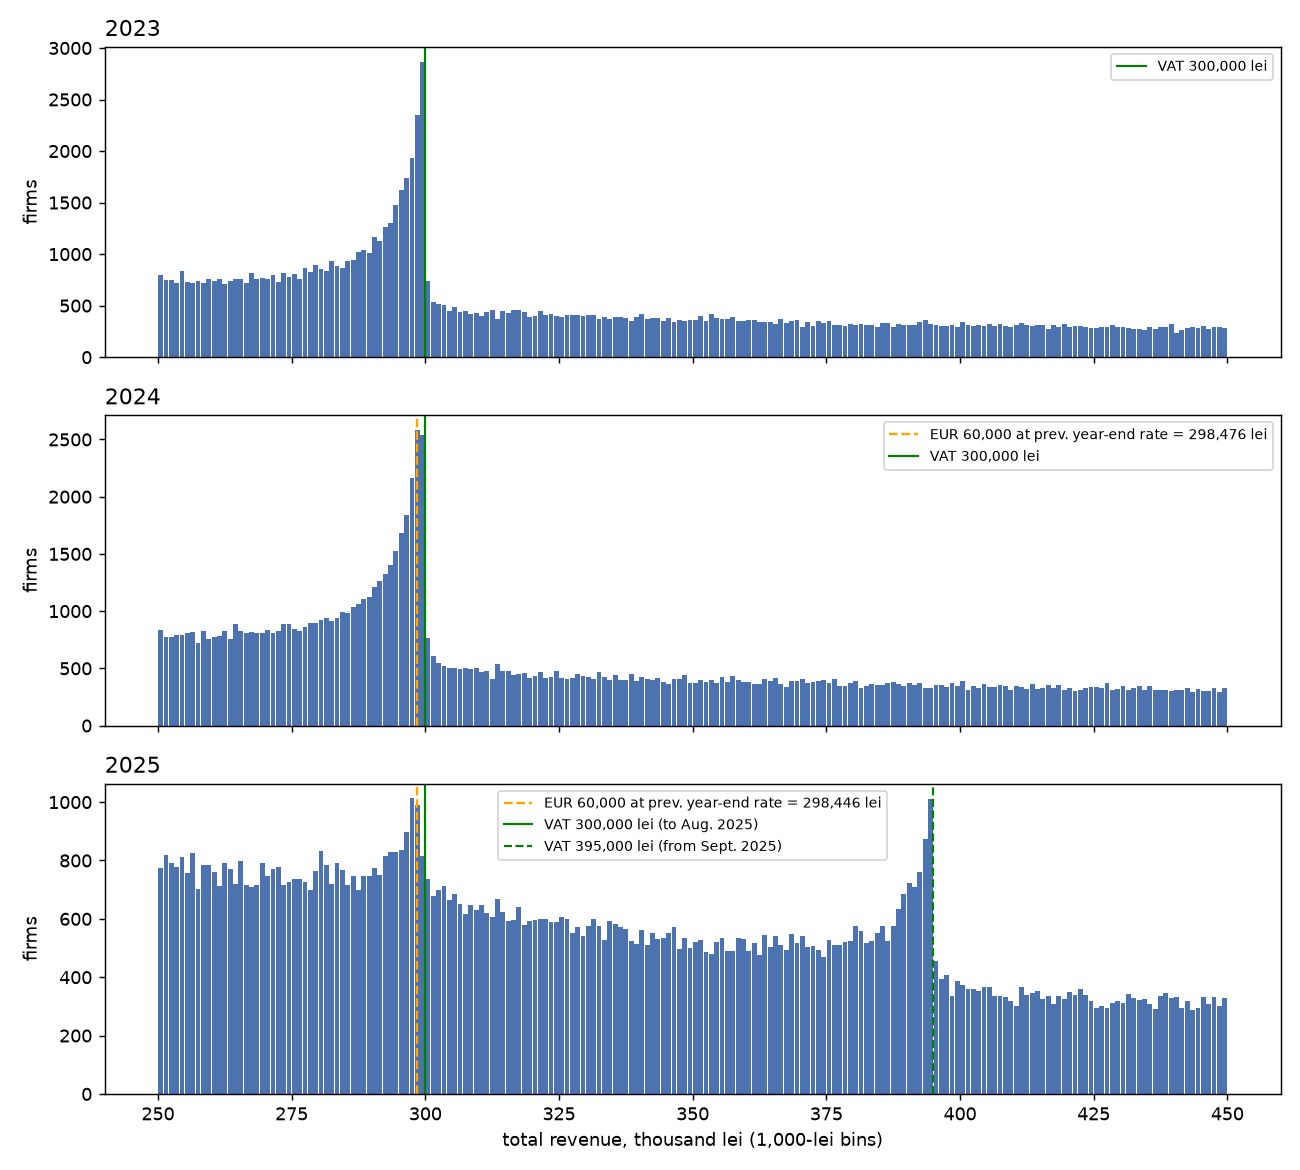
\includegraphics[width=0.8\textwidth]{boundary_60k_2023_2025.png}
\caption{Total revenue from 250,000 to 450,000 lei, 2023--2025, 1,000-lei bins, with the \euro{}60,000 rate boundary and the VAT thresholds.}\label{fig:boundary60k}
\end{figure}

\FloatBarrier
\subsection{The employee condition}

From 1 January 2023 a micro-enterprise must have at least one employee, tested at 31 December 2022; the condition was enacted in July 2022. Table~\ref{tab:emp} shows headcount among firms with revenue below \euro{}500,000: the share with exactly one employee rose from 31.9 percent in 2021 to 37.6 percent in 2022 and 40.7 percent in 2023, while the share with five or more fell. Table~\ref{tab:emptrans} follows zero-employee firms into the next year. In the 2021 to 2022 transition 22.3 percent of them moved to exactly one employee, against 11.1 to 11.3 percent in the two preceding transitions, or 20.3 percent when the sample is limited to firms present since 2020 to hold filing coverage fixed. Among zero-employee firms above \euro{}1,500,000, which the rule did not touch, the rate stayed at 5 to 6 percent throughout. This is about 20,000 additional one-employee firms. Of micro-enterprises that still had no employees at the end of 2022, 82 percent were registered for profit tax in 2023, and 15 percent had one employee and 3 percent two or more by the end of 2023. The hiring came in the year the rule was enacted; firms that had not hired by the deadline left the regime rather than hire afterwards. Among the 2022 hirers, 31 percent paid a blended rate that year, consistent with a hire during the year, and 12 percent the no-employee rate, consistent with a hire in the last quarter; in the 2021 placebo the shares are 14 and 19 percent. We read the response as compliance at the lowest cost rather than as job creation.
\FloatBarrier

\begin{table}[!tbp]\centering
\small
\caption{Employee counts among firms with revenue below \euro{}500,000 (\% of firms)}\label{tab:emp}
\resizebox{\linewidth}{!}{%
\begin{tabular}{lrrrrr}\toprule
Year & 0 employees & 1 & 2 & 5+ & Firms \\ \midrule
2019 & 33.6 & 28.7 & 13.9 & 11.8 & 555,050 \\
2020 & 33.4 & 30.6 & 13.4 & 11.2 & 575,855 \\
2021 & 35.1 & 31.9 & 12.1 & 10.2 & 558,724 \\
2022 & 31.1 & 37.6 & 11.9 & 9.1 & 616,503 \\
2023 & 28.7 & 40.7 & 12.5 & 8.3 & 640,536 \\
2024 & 30.6 & 40.8 & 12.2 & 7.3 & 686,605 \\
2025 & 32.6 & 40.5 & 11.8 & 6.4 & 655,235 \\
\bottomrule\end{tabular}}
\begin{minipage}{0.95\linewidth}\vspace{2pt}\footnotesize Average annual headcount as reported in the statements.\end{minipage}
\end{table}
\begin{table}[htbp]\centering
\small
\caption{Transitions of zero-employee firms (revenue below \euro{}500,000) into the next year, conditional on filing in both years (\%)}\label{tab:emptrans}
\resizebox{\linewidth}{!}{%
\begin{tabular}{lrrrr}\toprule
Year $t$ & Firms with 0 employees in $t$ & 1 employee in $t+1$ & 2+ in $t+1$ & Still 0 in $t+1$ \\ \midrule
2019 & 186,324 & 11.1 & 4.7 & 84.1 \\
2020 & 192,284 & 11.3 & 3.5 & 85.2 \\
2021 & 195,972 & 22.4 & 3.3 & 74.5 \\
2022 & 191,971 & 14.8 & 3.0 & 82.3 \\
2023 & 183,852 & 9.4 & 2.9 & 87.7 \\
2024 & 210,272 & 8.1 & 2.2 & 89.6 \\
\bottomrule\end{tabular}}
\begin{minipage}{0.95\linewidth}\vspace{2pt}\footnotesize The one-employee condition was enacted in July 2022 and tested at 31 December 2022. Filing coverage differs across years because some annual files are early uploads, so shares are conditional on a statement being present in $t+1$.\end{minipage}
\end{table}

\FloatBarrier
\subsection{Splitting}

Table~\ref{tab:split} compares limited-liability companies in the 5 percent below the ceiling with firms just above it, which are the same size, and with firms further below and well above. Pooled over 2018--2023, 2.7 percent of bunchers have an administrator who registered another firm in the previous eighteen months, against 2.0 percent of firms just above ($z = 4.3$, standard errors clustered by firm throughout) and 1.7 percent further below; 12.2 percent have another firm newly registered at their address, against 9.2 and 8.7 percent ($z = 8.6$). Dropping administrators without a birth date, whose key may merge namesakes, gives 2.4 against 1.7 percent, the same ratio. The share whose administrator runs any other firm, regardless of date, differs little between bunchers and firms just above ($z = 2.6$) and is similar for bunchers and firms well above the ceiling, so the timing measures rather than the level carry the information.

Bunchers are also younger than firms just above, 13 percent under three years old against 8 percent, and a young firm is more likely to have a recently registered sibling. Comparing within age bands (Appendix Table~\ref{tab:splitage}), bunchers exceed the just-above group in every band, and standardising to the bunchers' age distribution the premium is 23 percent on the administrator measure and 20 percent on the address measure. At the small ceilings of 2015--2017 the administrator measure shows no difference ($z = 1.5$, Table~\ref{tab:split} note).

The 2024 rules give two checks. From 2023 a person could hold over 25 percent in at most three micro-enterprises, and from 2024 in one, while the ceiling began to be tested on the combined revenue of linked enterprises. If the premium reflects splitting to stay under the ceiling, it should fall once splitting no longer helps, and combined revenue should start to bunch. The first holds on the administrator measure: bunchers and firms just above are at 1.4 percent each in 2024, against 2.0 and 1.6 in 2023; a gap remains on the address measure. The second does not: the combined revenue of firms sharing an administrator shows no excess mass at \euro{}500,000 in 2024, and firms inside such groups bunch individually at the same rate as single firms (Appendix Table~\ref{tab:groups}). Firms that lost the regime when the ceiling fell registered new firms at the same rate, relative to the band below, as placebo cohorts, so whatever splitting there is serves to stay under the line rather than to react to losing the regime. Either the aggregation rule was not enforced or noticed in its first year, or common administration is too weak a proxy for the ownership links the rule is written on; the evidence does not tell these apart, so the splitting result is a modest, robust correlation rather than an established mechanism. The register lists administrators as of 2026 rather than shareholders at the time, and the address measure will catch shared accountants' premises despite the exclusion of addresses hosting more than twenty firms.

\begin{landscape}
\begin{table}[htbp]\centering
\footnotesize
\caption{Sibling-firm indicators by position relative to the threshold, SRLs}\label{tab:split}
\resizebox{\linewidth}{!}{%
\begin{tabular}{llrrrrr}\toprule
Measure & Years & Bunchers (0--5\% below) & Just above (0--10\%) & 10--25\% below & 25--100\% above & $z$ \\ \midrule
Administrator registered another firm in prior 18 months & 2018--2023 & 2.71 & 1.98 & 1.72 & 1.91 & 4.5 \\
 & 2015--2017 & 1.59 & 1.37 & 1.38 & 1.48 & 1.5 \\
Another firm registered at the same address in prior 18 months & 2018--2023 & 12.23 & 9.18 & 8.72 & 8.37 & 9.1 \\
 & 2015--2017 & 7.16 & 5.35 & 6.04 & 5.37 & 6.4 \\
Administrator runs another firm (any date) & 2018--2023 & 17.09 & 15.88 & 15.16 & 17.46 & 3.0 \\
 & 2015--2017 & 12.42 & 11.38 & 11.13 & 12.15 & 2.7 \\
\bottomrule\end{tabular}}
\begin{minipage}{0.95\linewidth}\vspace{2pt}\footnotesize Pooled shares, \%. $z$ tests bunchers against firms just above the threshold. Administrators as recorded in the ONRC snapshot of 2 September 2026; persons administering more than 50 firms and addresses hosting more than 20 firms excluded.\end{minipage}
\end{table}
\end{landscape}

\FloatBarrier
\section{Conclusion}\label{sec:conc}

Romania's micro-enterprise ceiling moved six times in twelve years, and the distribution of reported firm revenue moved with it, to within a few thousand lei of the ceiling's value at the exchange rate written into the law. The variation identifies bunching without a fitted curve, under a stated and tested assumption, and at locations with no notch the estimator gives excess mass centred on zero, with a spread that every notch estimate exceeds. Excess mass is 2 to 8 percent of firms near the ceiling and 0.06 to 0.30 percent of all firms: the threshold is where the regime is visible, not where its cost lies. The channels point to a tax-saving motive concentrated in high-margin services. Bunching is two to three times stronger in professional and information services than in trade; reported margins rise by about 0.7 points when firms are moved onto the revenue tax and fall by 1 to 2 points when they are moved off it; firms took on a single employee in the year the employee condition was enacted or left the regime; and firms at the ceiling are somewhat more likely than equally sized and aged firms above it to have spun off a sibling firm, a premium that faded when linked enterprises began to be aggregated, even though combined revenue does not bunch. A static revenue simulation of the kind used in recent Romanian policy debate \citep{ban2023} assumes none of these responses; the estimates here are the behavioural inputs such simulations lack, and their aggregate size says the ceiling itself is a second-order concern. Turning the excess mass into an elasticity requires a model in which the tax base changes at the threshold, margins differ across firms and reported margins respond to the regime; the missing mass above the notch is too diffuse in these data to support the standard shortcut.

Four implications for design follow from the evidence, with the caveat that they concern the margins we can measure. First, the ceiling is the wrong lever. Moving it changes the behaviour of a few thousand firms and the tax bills of hundreds of thousands, so the choice of ceiling should be made on the intramarginal cost and on administrative grounds, not on the response at the threshold. Second, the regime's advantage is concentrated where margins are high. The activity list that taxes software, legal and medical firms at 3 percent regardless of revenue points in that direction, but the sectors with the largest bunching, professional, administrative, health and real-estate services, are only partly on it; a design that ties the rate to the margin, such as the minimum-tax structure that \citet{sharma2025dual} show dominates threshold systems, would remove both the notch and the incentive to report margins differently on the two sides of it. Third, side conditions that can be met with a single contract produce that contract: the employee condition created about 20,000 one-employee firms in the year it was enacted and pushed the rest out of the regime, and the linked-enterprise rule produced no bunching of combined revenue in its first year. Conditions should be written so that meeting them costs what the legislator intends. Fourth, any analysis of small-firm profitability in Romania, including the revenue simulations used in the policy debate, should condition on the tax regime, because reported margins move by 10 to 25 percent of their level when the regime changes and nothing else does.

\bibliographystyle{plainnat}
\begin{thebibliography}{99}
\bibitem[Almunia and L\'opez-Rodr\'iguez(2018)]{almunia2018} Almunia, M. and D. L\'opez-Rodr\'iguez (2018). Under the radar: The effects of monitoring firms on tax compliance. \emph{American Economic Journal: Economic Policy} 10(1), 1--38.
\bibitem[Asatryan and Peichl(2016)]{asatryan2016} Asatryan, Z. and A. Peichl (2016). Responses of firms to tax, administrative and accounting rules: Evidence from Armenia. ZEW Discussion Paper 16-065.
\bibitem[Bachas and Soto(2021)]{bachas2021} Bachas, P. and M. Soto (2021). Corporate taxation under weak enforcement. \emph{American Economic Journal: Economic Policy} 13(4), 36--71. doi:10.1257/pol.20180564.
\bibitem[Ban and Buciu(2023)]{ban2023} Ban, C. and P. Buciu (2023). \emph{Reforma fiscal\u{a}: propuneri pe termen scurt}. Bucharest: Friedrich-Ebert-Stiftung.
\bibitem[Best et al.(2015)]{best2015} Best, M., A. Brockmeyer, H. Kleven, J. Spinnewijn and M. Waseem (2015). Production versus revenue efficiency with limited tax capacity: Theory and evidence from Pakistan. \emph{Journal of Political Economy} 123(6), 1311--1355. doi:10.1086/683849.
\bibitem[Best and Kleven(2018)]{best2018} Best, M. and H. Kleven (2018). Housing market responses to transaction taxes: Evidence from notches and stimulus in the UK. \emph{Review of Economic Studies} 85(1), 157--193. doi:10.1093/restud/rdx032.
\bibitem[Blomquist et al.(2021)]{blomquist2021} Blomquist, S., W. Newey, A. Kumar and C.-Y. Liang (2021). On bunching and identification of the taxable income elasticity. \emph{Journal of Political Economy} 129(8), 2320--2343.
\bibitem[Boonzaaier et al.(2019)]{boonzaaier2019} Boonzaaier, W., J. Harju, T. Matikka and J. Pirttil\"a (2019). How do small firms respond to tax schedule discontinuities? Evidence from South African tax registers. \emph{International Tax and Public Finance} 26(5), 1104--1136. doi:10.1007/s10797-019-09550-z.
\bibitem[Chetty et al.(2011)]{chetty2011} Chetty, R., J. Friedman, T. Olsen and L. Pistaferri (2011). Adjustment costs, firm responses, and micro vs. macro labor supply elasticities: Evidence from Danish tax records. \emph{Quarterly Journal of Economics} 126(2), 749--804.
\bibitem[Consiliul Fiscal(2024)]{cf2024} Consiliul Fiscal (2024). \emph{Raport anual 2023}. Bucharest.
\bibitem[Dharmapala et al.(2011)]{dharmapala2011} Dharmapala, D., J. Slemrod and J. Wilson (2011). Tax policy and the missing middle: Optimal tax remittance with firm-level administrative costs. \emph{Journal of Public Economics} 95(9--10), 1036--1047.
\bibitem[Harju et al.(2019)]{harju2019vat} Harju, J., T. Matikka and T. Rauhanen (2019). Compliance costs vs. tax incentives: Why do entrepreneurs respond to size-based regulations? \emph{Journal of Public Economics} 173, 139--164.
\bibitem[IMF(2025)]{imf2025} International Monetary Fund (2025). \emph{Romania: Technical Assistance Report, High-Level Summary}. Washington, DC.
\bibitem[Kanbur and Keen(2014)]{kanbur2014} Kanbur, R. and M. Keen (2014). Thresholds, informality, and partitions of compliance. \emph{International Tax and Public Finance} 21(4), 536--559.
\bibitem[Kleven and Waseem(2013)]{kleven2013} Kleven, H. and M. Waseem (2013). Using notches to uncover optimization frictions and structural elasticities: Theory and evidence from Pakistan. \emph{Quarterly Journal of Economics} 128(2), 669--723.
\bibitem[Laz\u{a}r(2024)]{lazar2024} Laz\u{a}r, S. (2024). Effective tax rates and firm size under turnover tax: Evidence from a natural experiment on SMEs. \emph{Economics} 18(1), article 20220079. doi:10.1515/econ-2022-0079.
\bibitem[Liu et al.(2021)]{liu2021vat} Liu, L., B. Lockwood, M. Almunia and E. Tam (2021). VAT notches, voluntary registration, and bunching: Theory and UK evidence. \emph{Review of Economics and Statistics} 103(1), 151--164.
\bibitem[Marx(2024)]{marx2024} Marx, B. (2024). Dynamic bunching estimation with panel data. \emph{Journal of Econometric Methods} 13(2), 225--249. doi:10.1515/jem-2022-0031.
\bibitem[Sharma et al.(2025)]{sharma2025dual} Sharma, R., J. Slemrod, M. Stimmelmayr, J. Wilson and P. Choi (2025). Optimal dual-regime business tax systems. NBER Working Paper 34418. doi:10.3386/w34418.
\end{thebibliography}

\clearpage
\appendix
\section{Legal timeline}\label{app:legal}

The regime's parameters were changed by Ordinance 8/2013 (mandatory regime, \euro{}65,000, 3 percent, from 1 February 2013), Ordinance 102/2013 (consulting cap, 2014), Ordinance 50/2015 (\euro{}100,000 and employee-dependent rates, 2016), Ordinance 3/2017 (\euro{}500,000 from 1 February 2017), Ordinance 79/2017 (\euro{}1,000,000 from 2018, consulting cap abolished), Ordinance 25/2018 (capital and employee opt-out from April 2018), Ordinance 16/2022 of 15 July 2022 (\euro{}500,000, employee condition, three-firm rule, optional regime with permanent exit, from 2023) as amended by Law 370/2022 of 20 December 2022 (revenue test deferred to 2023 revenue), Law 296/2023 (\euro{}60,000 rate boundary and activity list, 2024), Ordinance 115/2023 (one-firm rule and linked-enterprise aggregation, 2024), Ordinance 156/2024 of 31 December 2024 (\euro{}250,000 for 2025, \euro{}100,000 for 2026, consulting cap abolished), Ordinance 89/2025 (flat 1 percent from 2026) and Ordinance 8/2026 (turnover base from 2026). Exchange-rate provisions: Article 47(1)(c) for the year-end test and Article 52 for the in-year test of Law 227/2015, and before 2016 Article 112$^6$ of Law 571/2003 with its implementing norms; in every version the in-year test uses the BNR rate at the close of the previous financial year. VAT thresholds: Article 310 of Law 227/2015 as amended by Law 72/2018 (300,000 lei from 1 April 2018) and Ordinance 22/2025 (395,000 lei from 1 September 2025). A full table with Monitorul Oficial references accompanies the replication files. Policy assessments of the regime are in \citet{imf2025}, \citet{cf2024}, \citet{ban2023} and \citet{lazar2024}.

\FloatBarrier
\section{Additional tables}\label{app:tables}

Table~\ref{tab:controls} lists the admissible control years for each notch with the matched revenue and its distance to the nearest notch. Table~\ref{tab:robustextra} gives the robustness checks not shown in the body. Three further checks are not tabulated: the excess counts vary across the 3, 5 and 8 percent region definitions by 6 to 50 percent, mostly at the two extra notches where the bunching region is wide; dropping hospitality firms, which faced no revenue ceiling in 2023, raises the 2023 estimate from 2.99 to 3.14, and hospitality firms alone show 0.58; and newly created firms make up 11 percent of the 2023 excess, against 7 percent in 2021 and 13 percent in 2024, so entry at the threshold is a small part of it. Table~\ref{tab:transition} gives the origin of firms just below \euro{}500,000 in the notch year and in placebo years. Table~\ref{tab:eventstudy} gives the wide-band event study that motivates the narrowed bands in the body. Tables~\ref{tab:splitage} and \ref{tab:groups} give the age-band comparison and the combined-revenue test for the splitting section. Table~\ref{tab:elasticity} gives the reduced-form elasticities discussed in Section~\ref{sec:results}.

\begin{table}[tbp]\centering
\footnotesize
\caption{Admissible control years, matched locations and distance to the nearest notch}\label{tab:controls}
\resizebox{\linewidth}{!}{%
\begin{tabular}{lp{11.5cm}}\toprule
Notch & Control year: matched revenue $L^*_c$ (distance to nearest notch in that year) \\ \midrule
2014: in-year, \euro{}65,000 & 2016: 0.32M (32\%); 2017: 0.33M (34\%); 2022: 0.44M (31\%); 2023: 0.46M (35\%); 2024: 0.47M (36\%) \\
2015: in-year, \euro{}65,000 & 2016: 0.30M (26\%); 2017: 0.30M (27\%); 2023: 0.43M (30\%); 2024: 0.43M (31\%) \\
2016: in-year, \euro{}100,000 & 2014: 0.42M (30\%); 2015: 0.47M (38\%); 2017: 0.48M (54\%); 2018: 0.50M (40\%); 2019: 0.52M (42\%); 2020: 0.49M (39\%); 2021: 0.57M (47\%); 2022: 0.62M (52\%); 2023: 0.66M (54\%); 2024: 0.66M (54\%) \\
2017: in-year, \euro{}500,000 & 2014: 2.09M (86\%); 2015: 2.25M (87\%); 2016: 2.25M (80\%); 2018: 2.42M (88\%); 2019: 2.50M (86\%); 2020: 2.39M (88\%); 2021: 2.80M (74\%); 2025: 3.13M (60\%) \\
2018: in-year, \euro{}1,000,000 & 2014: 4.19M (93\%); 2015: 4.49M (94\%); 2016: 4.44M (90\%); 2017: 4.54M (50\%); 2023: 5.83M (58\%); 2024: 5.88M (58\%); 2025: 6.26M (80\%) \\
2019: in-year, \euro{}1,000,000 & 2014: 4.12M (93\%); 2015: 4.41M (93\%); 2016: 4.37M (90\%); 2017: 4.46M (49\%); 2023: 5.73M (57\%); 2024: 5.79M (57\%); 2025: 6.16M (80\%) \\
2020: in-year, \euro{}1,000,000 & 2014: 4.42M (93\%); 2015: 4.73M (94\%); 2016: 4.69M (90\%); 2017: 4.76M (52\%); 2023: 6.15M (60\%); 2024: 6.21M (60\%); 2025: 6.60M (81\%) \\
2021: in-year, \euro{}1,000,000 & 2014: 3.92M (93\%); 2015: 4.19M (93\%); 2016: 4.15M (89\%); 2017: 4.24M (46\%); 2023: 5.44M (54\%); 2024: 5.48M (55\%); 2025: 5.84M (79\%) \\
2022: in-year, \euro{}1,000,000 & 2014: 3.56M (92\%); 2015: 3.82M (92\%); 2016: 3.79M (88\%); 2017: 3.87M (41\%); 2023: 4.94M (50\%); 2024: 5.01M (50\%); 2025: 5.32M (77\%) \\
2023: in-year, \euro{}500,000 & 2014: 1.79M (84\%); 2015: 1.94M (85\%); 2016: 1.94M (77\%); 2018: 2.09M (86\%); 2019: 2.16M (86\%); 2020: 2.07M (86\%); 2021: 2.42M (88\%); 2025: 2.70M (54\%) \\
2024: in-year, \euro{}500,000 & 2014: 1.75M (83\%); 2015: 1.91M (85\%); 2016: 1.90M (76\%); 2018: 2.05M (85\%); 2019: 2.12M (86\%); 2020: 2.03M (85\%); 2021: 2.37M (87\%); 2025: 2.65M (53\%) \\
2025: in-year, \euro{}250,000 & 2014: 0.82M (64\%); 2015: 0.90M (68\%); 2016: 0.89M (49\%); 2017: 0.92M (76\%); 2018: 0.97M (69\%); 2019: 1.01M (70\%); 2020: 0.96M (69\%); 2021: 1.11M (73\%); 2022: 1.21M (75\%); 2023: 1.25M (76\%); 2024: 1.23M (76\%) \\
2022: announced, \euro{}500,000 & 2014: 1.69M (83\%); 2015: 1.84M (84\%); 2016: 1.83M (75\%); 2018: 1.97M (85\%); 2019: 2.05M (85\%); 2020: 1.96M (85\%); 2021: 2.28M (87\%); 2025: 2.56M (51\%) \\
2025: year-end, \euro{}100,000 & 2016: 0.34M (31\%); 2017: 0.35M (37\%); 2021: 0.42M (29\%); 2022: 0.46M (35\%); 2023: 0.49M (39\%); 2024: 0.50M (40\%) \\
\bottomrule\end{tabular}}
\begin{minipage}{0.95\linewidth}\vspace{2pt}\footnotesize $L^*_c$ = revenue at the notch's quantile in the control year. Distance = $|n/L^*_c - 1|$ for the nearest known notch $n$ of that year (micro ceiling, future ceiling, \euro{}60,000 boundary or VAT threshold); admissible if above 25\%. The closest cases are 26--34\%.\end{minipage}
\end{table}
\begin{table}[!tbp]\centering
\small
\caption{Further robustness checks of the difference-in-bunching estimates}\label{tab:robustextra}
\resizebox{\linewidth}{!}{%
\begin{tabular}{lrrrrrrr}\toprule
Notch & $b$ & Quantile-corrected & Pre-years only & Post-years only & Continuing firms & $n$ continuing & Jackknife SE \\ \midrule
2014: in-year, \euro{}65,000 & 1.15 & 1.14 & -- & 1.15 & 1.15 & 31,696 & 0.04 \\
2015: in-year, \euro{}65,000 & 1.71 & 1.70 & -- & 1.71 & 1.71 & 30,382 & 0.02 \\
2016: in-year, \euro{}100,000 & 1.56 & 1.56 & 1.30 & 1.63 & 1.45 & 29,322 & 0.08 \\
2017: in-year, \euro{}500,000 & 0.76 & 0.77 & 0.62 & 0.85 & 0.72 & 16,321 & 0.05 \\
2018: in-year, \euro{}1,000,000 & 1.41 & 1.36 & 1.44 & 1.37 & 1.35 & 11,010 & 0.04 \\
2019: in-year, \euro{}1,000,000 & 1.67 & 1.75 & 1.64 & 1.70 & 1.58 & 12,513 & 0.06 \\
2020: in-year, \euro{}1,000,000 & 1.75 & 1.87 & 1.64 & 1.90 & 1.67 & 11,535 & 0.09 \\
2021: in-year, \euro{}1,000,000 & 2.15 & 2.19 & 2.23 & 2.04 & 2.08 & 13,668 & 0.08 \\
2022: in-year, \euro{}1,000,000 & 1.92 & 1.97 & 1.82 & 2.05 & 1.77 & 14,756 & 0.09 \\
2023: in-year, \euro{}500,000 & 2.99 & 2.99 & 3.02 & 2.82 & 2.80 & 26,100 & 0.05 \\
2024: in-year, \euro{}500,000 & 1.62 & 1.65 & 1.64 & 1.52 & 1.58 & 24,967 & 0.04 \\
2025: in-year, \euro{}250,000 & 0.73 & 0.72 & 0.73 & -- & 0.61 & 35,470 & 0.04 \\
2022: announced, \euro{}500,000 & 0.80 & 0.79 & 0.80 & 0.83 & 0.83 & 21,379 & 0.03 \\
2025: year-end, \euro{}100,000 & 1.47 & 1.47 & 1.47 & -- & 1.43 & 51,879 & 0.04 \\
\bottomrule\end{tabular}}
\begin{minipage}{0.95\linewidth}\vspace{2pt}\footnotesize Quantile-corrected: control quantile shifted down by $B/N_t$. Pre/post: only control years before/after the treated year. Continuing: firms with positive revenue in $t-1$, $t$ and $t+1$. Jackknife SE over control years.\end{minipage}
\end{table}
\begin{table}[tbp]\centering
\small
\caption{Origin of firms just below \euro{}500,000: share that was above \euro{}500,000 the year before}\label{tab:transition}
\resizebox{\linewidth}{!}{%
\begin{tabular}{llrrrrrr}\toprule
Year & Status & Firms 0--6\% below & \% above \euro{}500k in $t-1$ & \% in 120--200\% band in $t-1$ & Firms 14--20\% below & \% above in $t-1$ & Ratio \\ \midrule
2019 & placebo & 2,999 & 23.6 & 8.3 & 3,922 & 12.3 & 1.92 \\
2020 & placebo & 2,895 & 40.7 & 17.5 & 3,817 & 25.0 & 1.63 \\
2021 & placebo & 3,058 & 19.4 & 7.3 & 3,999 & 9.9 & 1.96 \\
2023 & notch year & 6,646 & 29.6 & 15.1 & 5,166 & 16.6 & 1.78 \\
2024 & post-transition & 5,659 & 21.7 & 7.3 & 5,403 & 14.0 & 1.55 \\
\bottomrule\end{tabular}}
\begin{minipage}{0.95\linewidth}\vspace{2pt}\footnotesize Positions relative to \euro{}500,000 at the previous year-end rate in every year, whether or not it was a threshold. Ratio = bunchers' share from above divided by the comparison group's share.\end{minipage}
\end{table}
\begin{table}[!tbp]\centering
\footnotesize
\caption{Reported pre-tax margins around regime switches induced by ceiling changes}\label{tab:eventstudy}
\resizebox{\linewidth}{!}{%
\begin{tabular}{lllllll}\toprule
Year & Micro share T / C (\%) & Median margin T (\%) & Median margin C (\%) & DiD median (pp) & DiD mean (pp) & Median revenue T / C (k\euro{}) \\ \midrule
\multicolumn{7}{l}{\emph{2018 increase: (500k, 1M] vs (1M, 2M] on 2017 revenue}} \\
2015 & 15 / 14 & 5.39 & 5.07 & -0.32 & -0.39 & 559 / 1,108 \\
2016 & 14 / 14 & 5.80 & 5.41 & -0.25 & -0.43 & 628 / 1,232 \\
2017 & 27 / 15 & 6.00 & 5.36 & +0.00 & +0.00 & 684 / 1,351 \\
2018 & 72 / 18 & 6.37 & 4.93 & +0.80 & +0.85 & 728 / 1,438 \\
2019 & 61 / 22 & 6.22 & 4.89 & +0.69 & +0.65 & 746 / 1,466 \\
2020 & 58 / 26 & 6.07 & 5.06 & +0.37 & -0.08 & 675 / 1,342 \\
\multicolumn{7}{l}{\emph{2023 cut: (500k, 1M] vs (1M, 2M] on 2022 revenue}} \\
2020 & 74 / 51 & 9.84 & 7.70 & -0.70 & -1.14 & 462 / 912 \\
2021 & 75 / 48 & 11.87 & 9.36 & -0.33 & -0.51 & 576 / 1,090 \\
2022 & 75 / 36 & 11.76 & 8.92 & +0.00 & +0.00 & 696 / 1,351 \\
2023 & 55 / 24 & 8.40 & 6.69 & -1.13 & -1.49 & 676 / 1,358 \\
2024 & 24 / 18 & 6.43 & 5.69 & -2.10 & -2.49 & 691 / 1,381 \\
2025 & 18 / 17 & 5.80 & 5.35 & -2.39 & -3.22 & 686 / 1,366 \\
\multicolumn{7}{l}{\emph{Placebo: same bands on 2019 revenue, no regime change}} \\
2017 & 46 / 24 & 7.35 & 5.66 & -1.47 & -1.60 & 533 / 1,099 \\
2018 & 74 / 37 & 8.24 & 5.82 & -0.74 & -0.88 & 621 / 1,249 \\
2019 & 71 / 26 & 8.95 & 5.79 & +0.00 & +0.00 & 692 / 1,364 \\
2020 & 70 / 21 & 7.85 & 5.54 & -0.85 & -0.98 & 640 / 1,270 \\
2021 & 66 / 29 & 9.43 & 6.63 & -0.36 & -1.17 & 718 / 1,421 \\
\bottomrule\end{tabular}}
\begin{minipage}{0.95\linewidth}\vspace{2pt}\footnotesize Balanced panels of firms with positive revenue in every year shown. T = firms whose base-year revenue placed them in the band that changed regime; C = firms in the band above that did not. DiD = change in T minus change in C relative to the base year (2017, 2022, 2019). Margins are pre-tax profit over revenue, winsorised at $\pm$1. The placebo shows the drift induced by selecting on base-year revenue alone.\end{minipage}
\end{table}
\begin{table}[tbp]\centering
\small
\caption{Sibling-firm indicators by firm age, bunchers versus firms just above the threshold, pooled 2018--2023 (\%)}\label{tab:splitage}
\resizebox{\linewidth}{!}{%
\begin{tabular}{lrrrrrr}\toprule
Firm age (years) & Bunchers, $n$ & Just above, $n$ & Admin.\ new firm: bunchers & just above & Same-address new firm: bunchers & just above \\ \midrule
0-2 & 2,166 & 1,482 & 6.97 & 5.47 & 26.13 & 20.51 \\
3-5 & 2,544 & 2,332 & 3.26 & 2.57 & 18.20 & 16.51 \\
6-10 & 3,662 & 3,826 & 2.48 & 2.12 & 13.68 & 11.53 \\
11+ & 8,158 & 10,187 & 1.50 & 1.25 & 6.09 & 4.96 \\
\bottomrule\end{tabular}}
\begin{minipage}{0.95\linewidth}\vspace{2pt}\footnotesize Age = year minus year of registration in the trade register. Standardising the just-above group to the bunchers' age distribution gives 2.70 versus 2.20 (administrator measure, +23\%) and 12.26 versus 10.23 (address measure, +20\%).\end{minipage}
\end{table}
\begin{landscape}
\begin{table}[!tbp]\centering
\footnotesize
\caption{Bunching of combined revenue of firms sharing an administrator, and firm-level bunching inside groups}\label{tab:groups}
\resizebox{\linewidth}{!}{%
\begin{tabular}{lrrrrrr}\toprule
Year & Groups (2--5 SRLs, one administrator) & Groups in window & $b$, combined revenue at \euro{}500k & Excess groups & Firms in groups: \% in 5\% below own notch & Single firms: same \\ \midrule
2021 & 13,563 & 970 & 0.11 & 3 & 19.5 & 18.1 \\
2022 & 15,156 & 1,118 & 0.58 & 16 & 18.9 & 17.5 \\
2023 & 15,860 & 1,304 & 0.90 & 29 & 21.5 & 20.1 \\
2024 & 17,323 & 1,417 & 0.07 & 3 & 16.2 & 16.9 \\
2025 & 18,044 & 1,335 & 0.62 & 20 & 15.8 & 14.5 \\
\bottomrule\end{tabular}}
\begin{minipage}{0.95\linewidth}\vspace{2pt}\footnotesize From 2024 the ceiling is tested on the combined revenue of linked enterprises. Combined revenue of each administrator's firms, window $\pm$20\% around \euro{}500,000 at the previous year-end rate, controls = same-quantile density of combined revenue in 2019--2022 excluding years where the individual \euro{}1M notch is within 25\%. Last two columns: share of firms within 20\% of that year's individual notch that sit in the 5\% just below it.\end{minipage}
\end{table}
\end{landscape}
\begin{table}[htbp]\centering
\footnotesize
\caption{Reduced-form elasticities under the Kleven--Waseem approximation, reported for completeness}\label{tab:elasticity}
\resizebox{\linewidth}{!}{%
\begin{tabular}{lrrrrrrr}\toprule
Notch & $\tau$ & median buncher margin & $\Delta t$ (pp) & $\Delta z^*/z^*$ from $b$ (\%) & $e$ from $b$ & hole width (\%) & $e$ from hole \\ \midrule
2014: in-year, \euro{}65,000 & 3\% & 0.160 & -0.44 & 1.15 & undefined (dt<=0) & -- & undefined (dt<=0) \\
2015: in-year, \euro{}65,000 & 3\% & 0.169 & -0.30 & 1.71 & undefined (dt<=0) & 20 & undefined (dt<=0) \\
2016: in-year, \euro{}100,000 & 3\% & 0.134 & -0.86 & 1.56 & undefined (dt<=0) & 19 & undefined (dt<=0) \\
2017: in-year, \euro{}500,000 & 1\% & 0.089 & +0.42 & 0.76 & 0.007 & 20 & 4.67 \\
2018: in-year, \euro{}1,000,000 & 1\% & 0.106 & +0.70 & 1.41 & 0.014 & 18 & 2.3 \\
2019: in-year, \euro{}1,000,000 & 1\% & 0.117 & +0.87 & 1.67 & 0.016 & 18 & 1.84 \\
2020: in-year, \euro{}1,000,000 & 1\% & 0.132 & +1.11 & 1.75 & 0.014 & 19 & 1.61 \\
2021: in-year, \euro{}1,000,000 & 1\% & 0.160 & +1.56 & 2.15 & 0.015 & 19 & 1.15 \\
2022: in-year, \euro{}1,000,000 & 1\% & 0.166 & +1.66 & 1.92 & 0.011 & 20 & 1.2 \\
2023: in-year, \euro{}500,000 & 1\% & 0.200 & +2.20 & 2.99 & 0.02 & -- & hole not identified \\
2024: in-year, \euro{}500,000 & 3\% & 0.151 & -0.58 & 1.62 & undefined (dt<=0) & 19 & undefined (dt<=0) \\
2025: in-year, \euro{}250,000 & 3\% & 0.135 & -0.84 & 0.73 & undefined (dt<=0) & 20 & undefined (dt<=0) \\
2022: announced, \euro{}500,000 & 1\% & 0.140 & +1.24 & 0.80 & 0.003 & 18 & 1.29 \\
2025: year-end, \euro{}100,000 & 3\% & 0.234 & +0.74 & 1.47 & 0.014 & 20 & 2.61 \\
\bottomrule\end{tabular}}
\begin{minipage}{0.95\linewidth}\vspace{2pt}\footnotesize $\Delta t = 0.16 \times \text{margin} - \tau$ is the change in the average tax rate on revenue at the notch for a firm with the median reported margin of bunchers; $e = (\Delta z^*/z^*)^2 / (2\Delta t/(1-\tau))$. Two proxies for $\Delta z^*/z^*$: $b$ with 1\% bins, and the width above the notch at which the cumulative deficit offsets the excess (the hole), which is not reached before the window edge in most years. The proxies differ by three orders of magnitude and $\Delta t \le 0$ in the 3\% years, which is why the text does not rely on these numbers.\end{minipage}
\end{table}

\FloatBarrier
\clearpage
\section{Additional figures}\label{app:figures}

\begin{figure}[!tbp]\centering
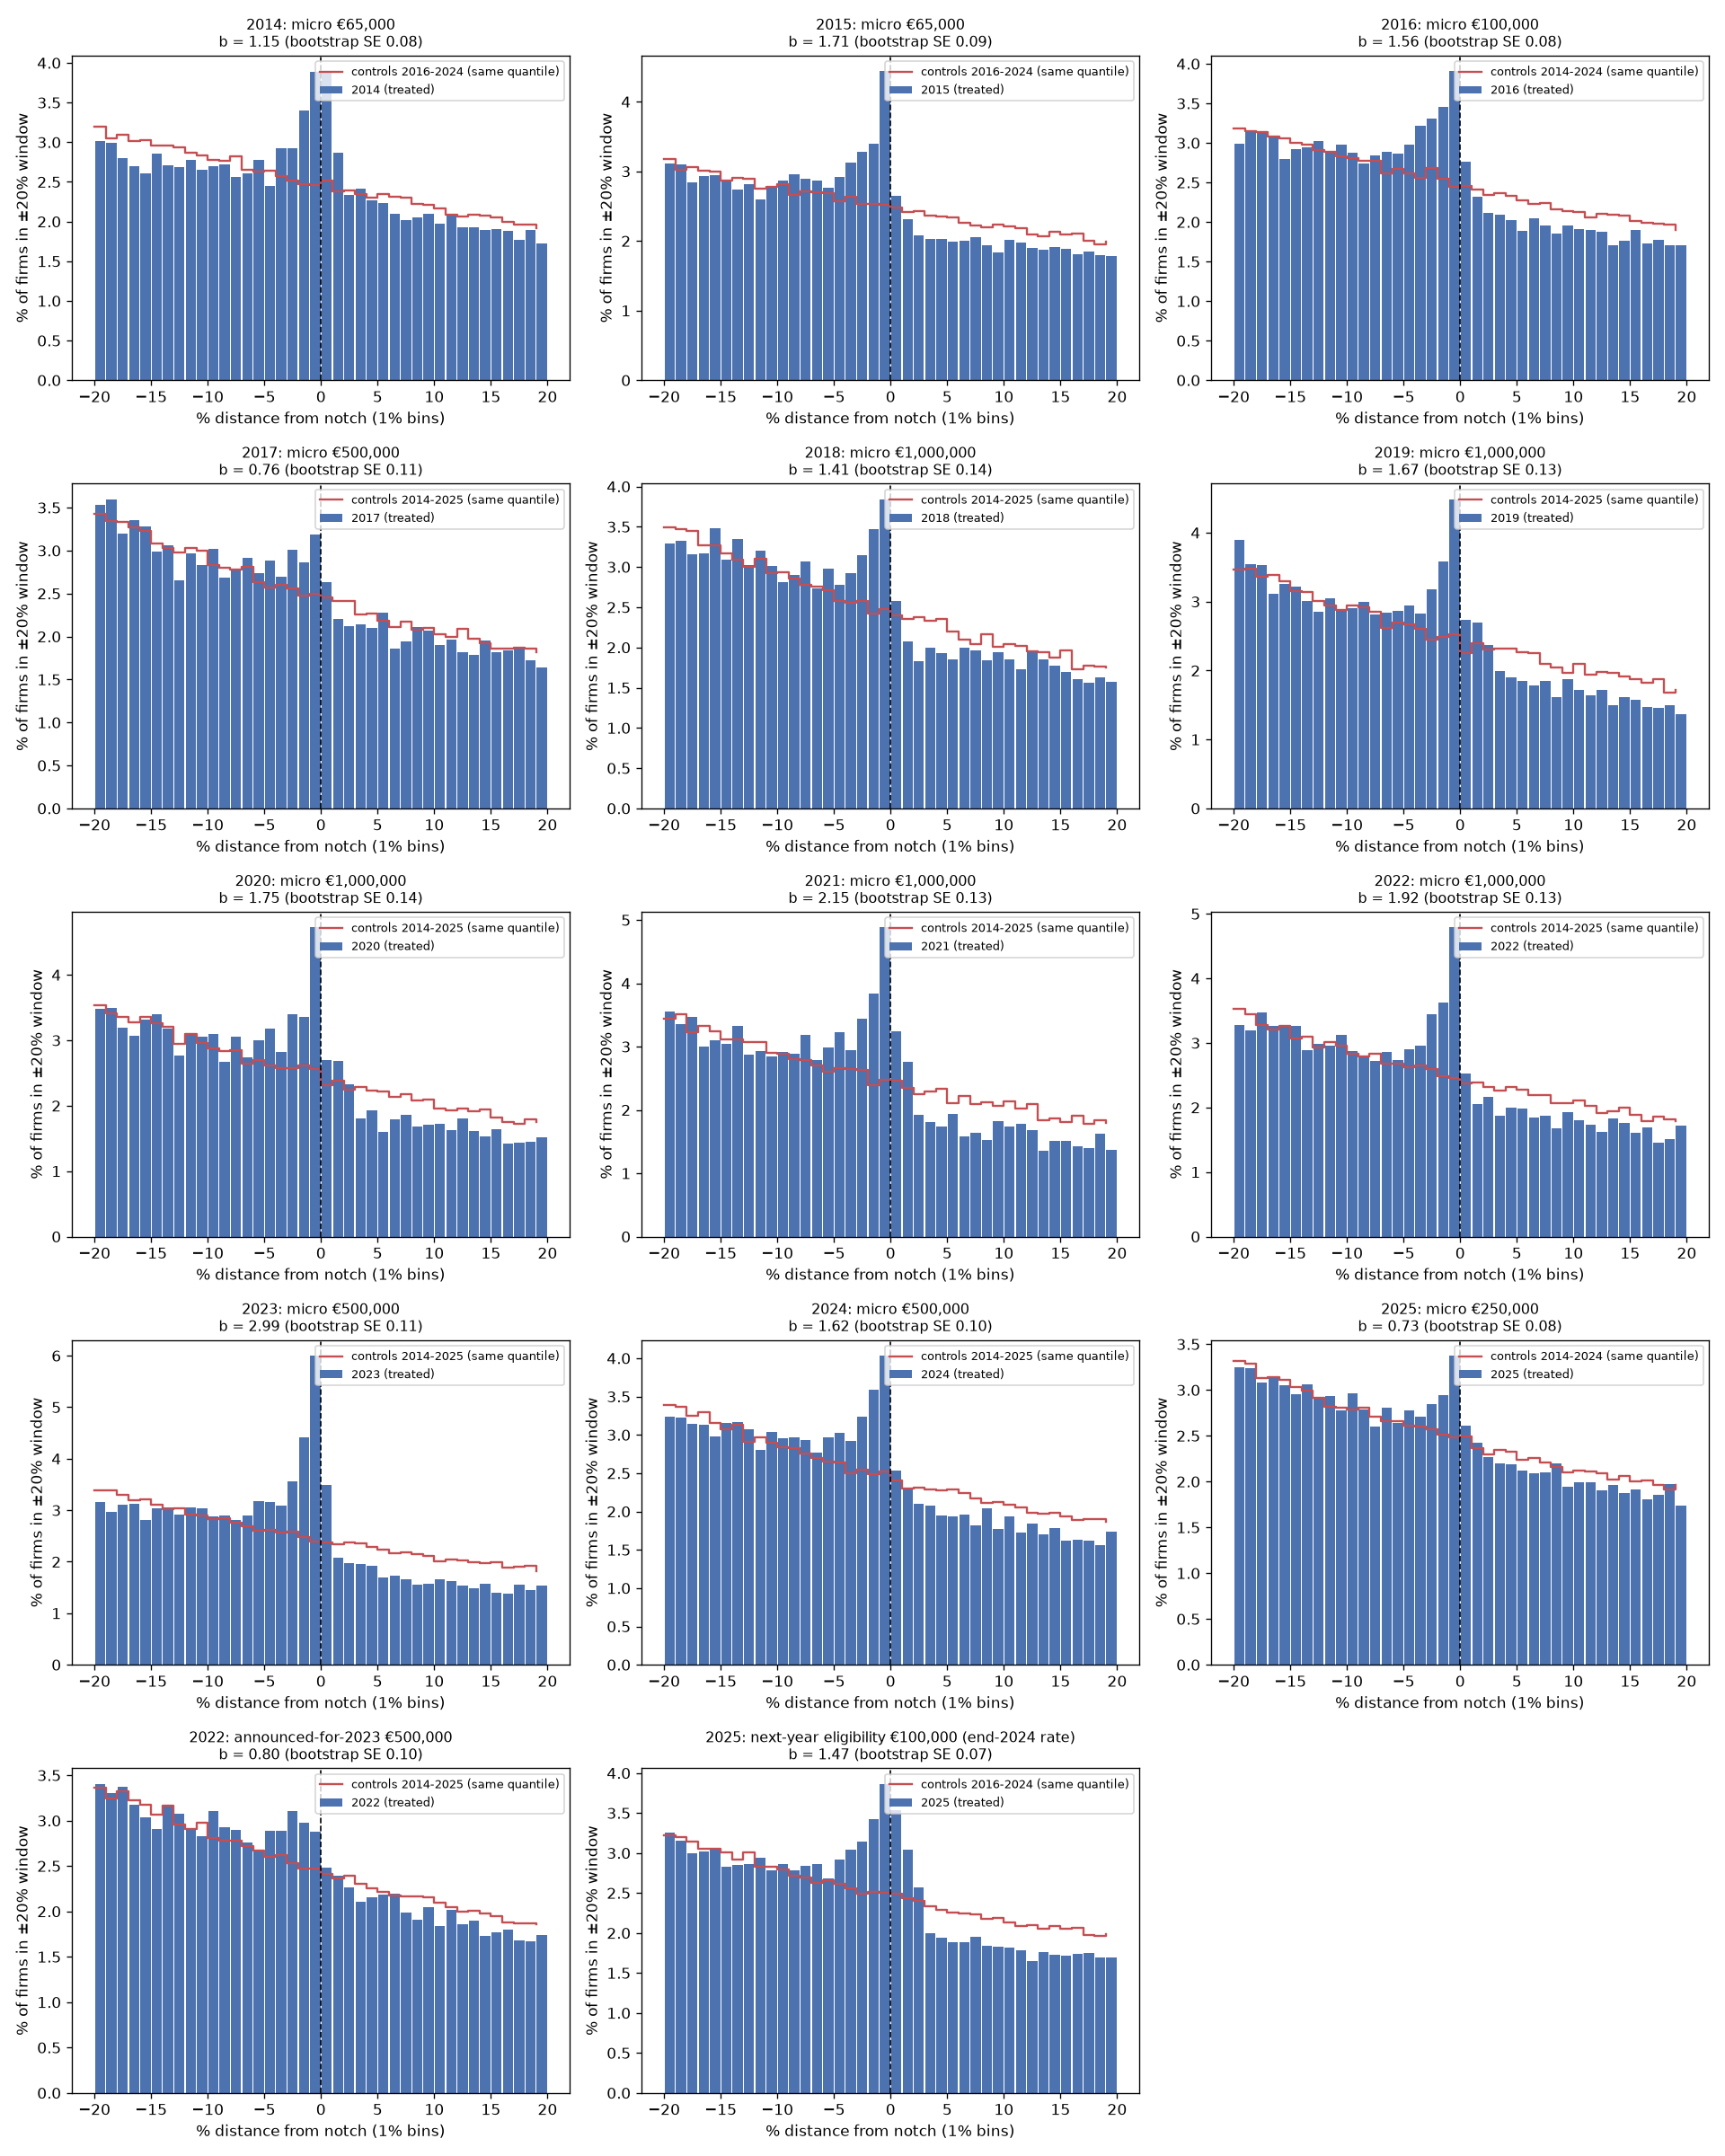
\includegraphics[width=\textwidth]{diff_in_bunching.png}
\caption{Treated-year density (bars) and same-quantile control density (line) around each of the fourteen notches, bins of 1 percent of the notch location.}\label{fig:dibfull}
\end{figure}

\begin{figure}[!tbp]\centering
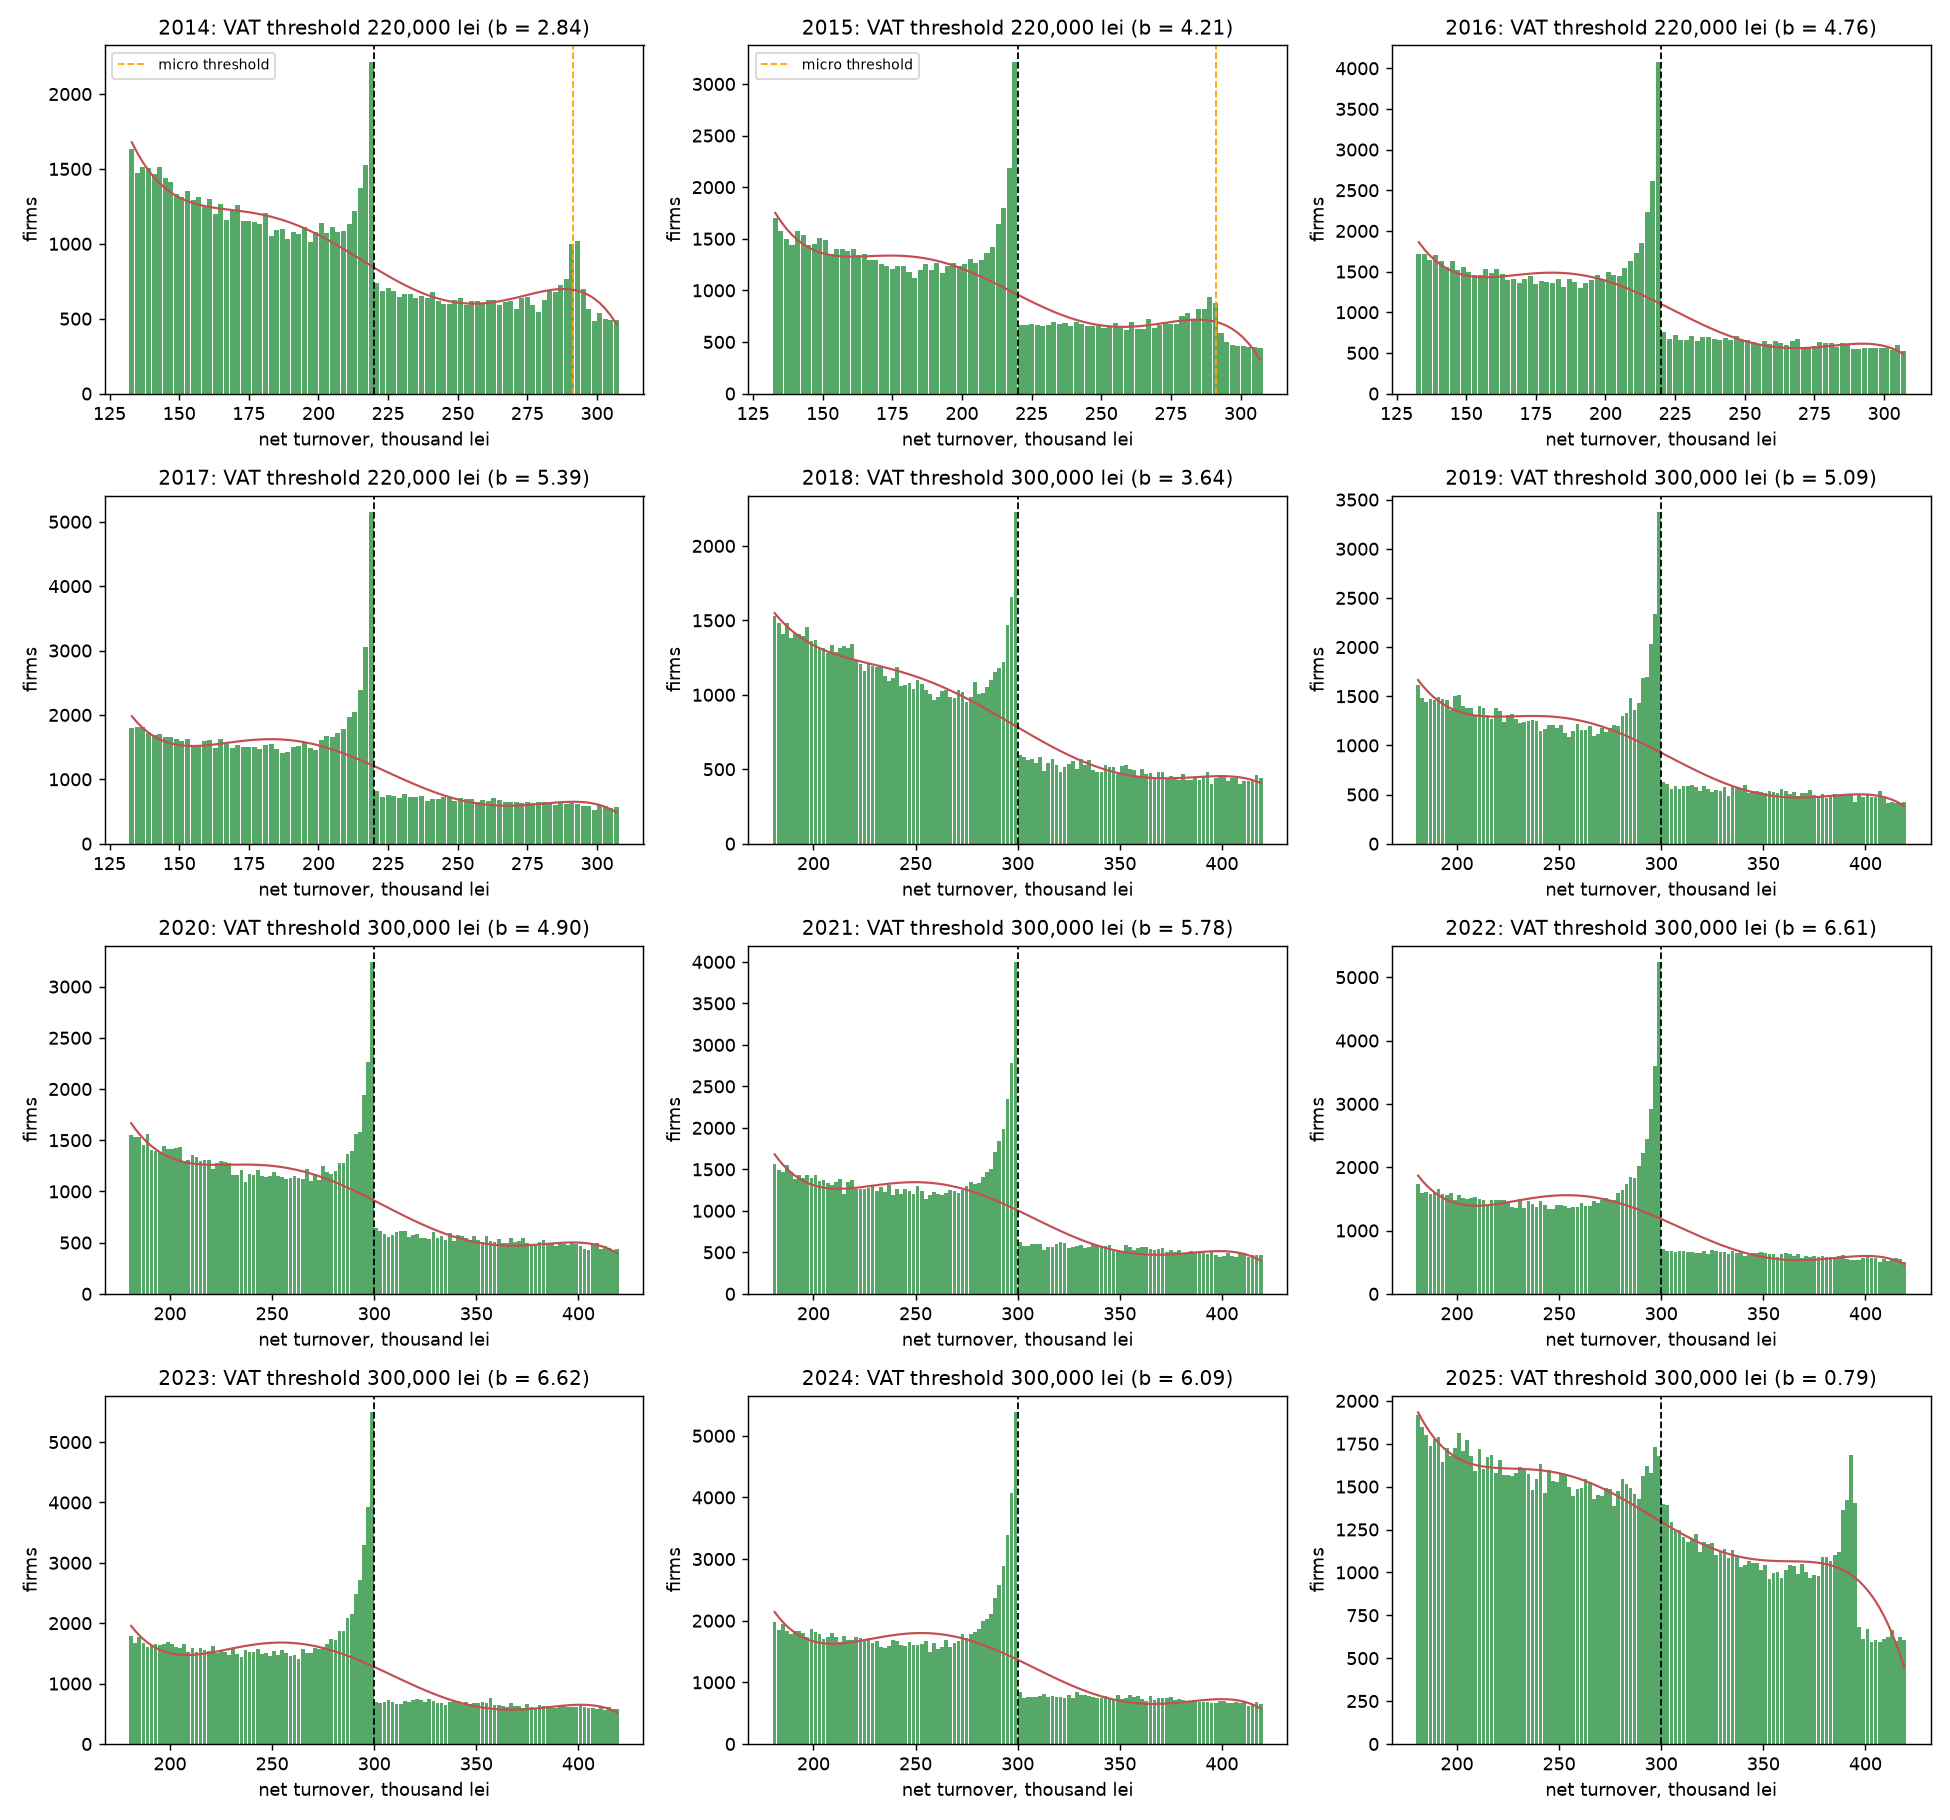
\includegraphics[width=\textwidth]{vat_threshold_panels.png}
\caption{Net turnover around the VAT registration threshold, 2,000-lei bins, with a polynomial counterfactual.}\label{fig:vat}
\end{figure}

\begin{figure}[!tbp]\centering
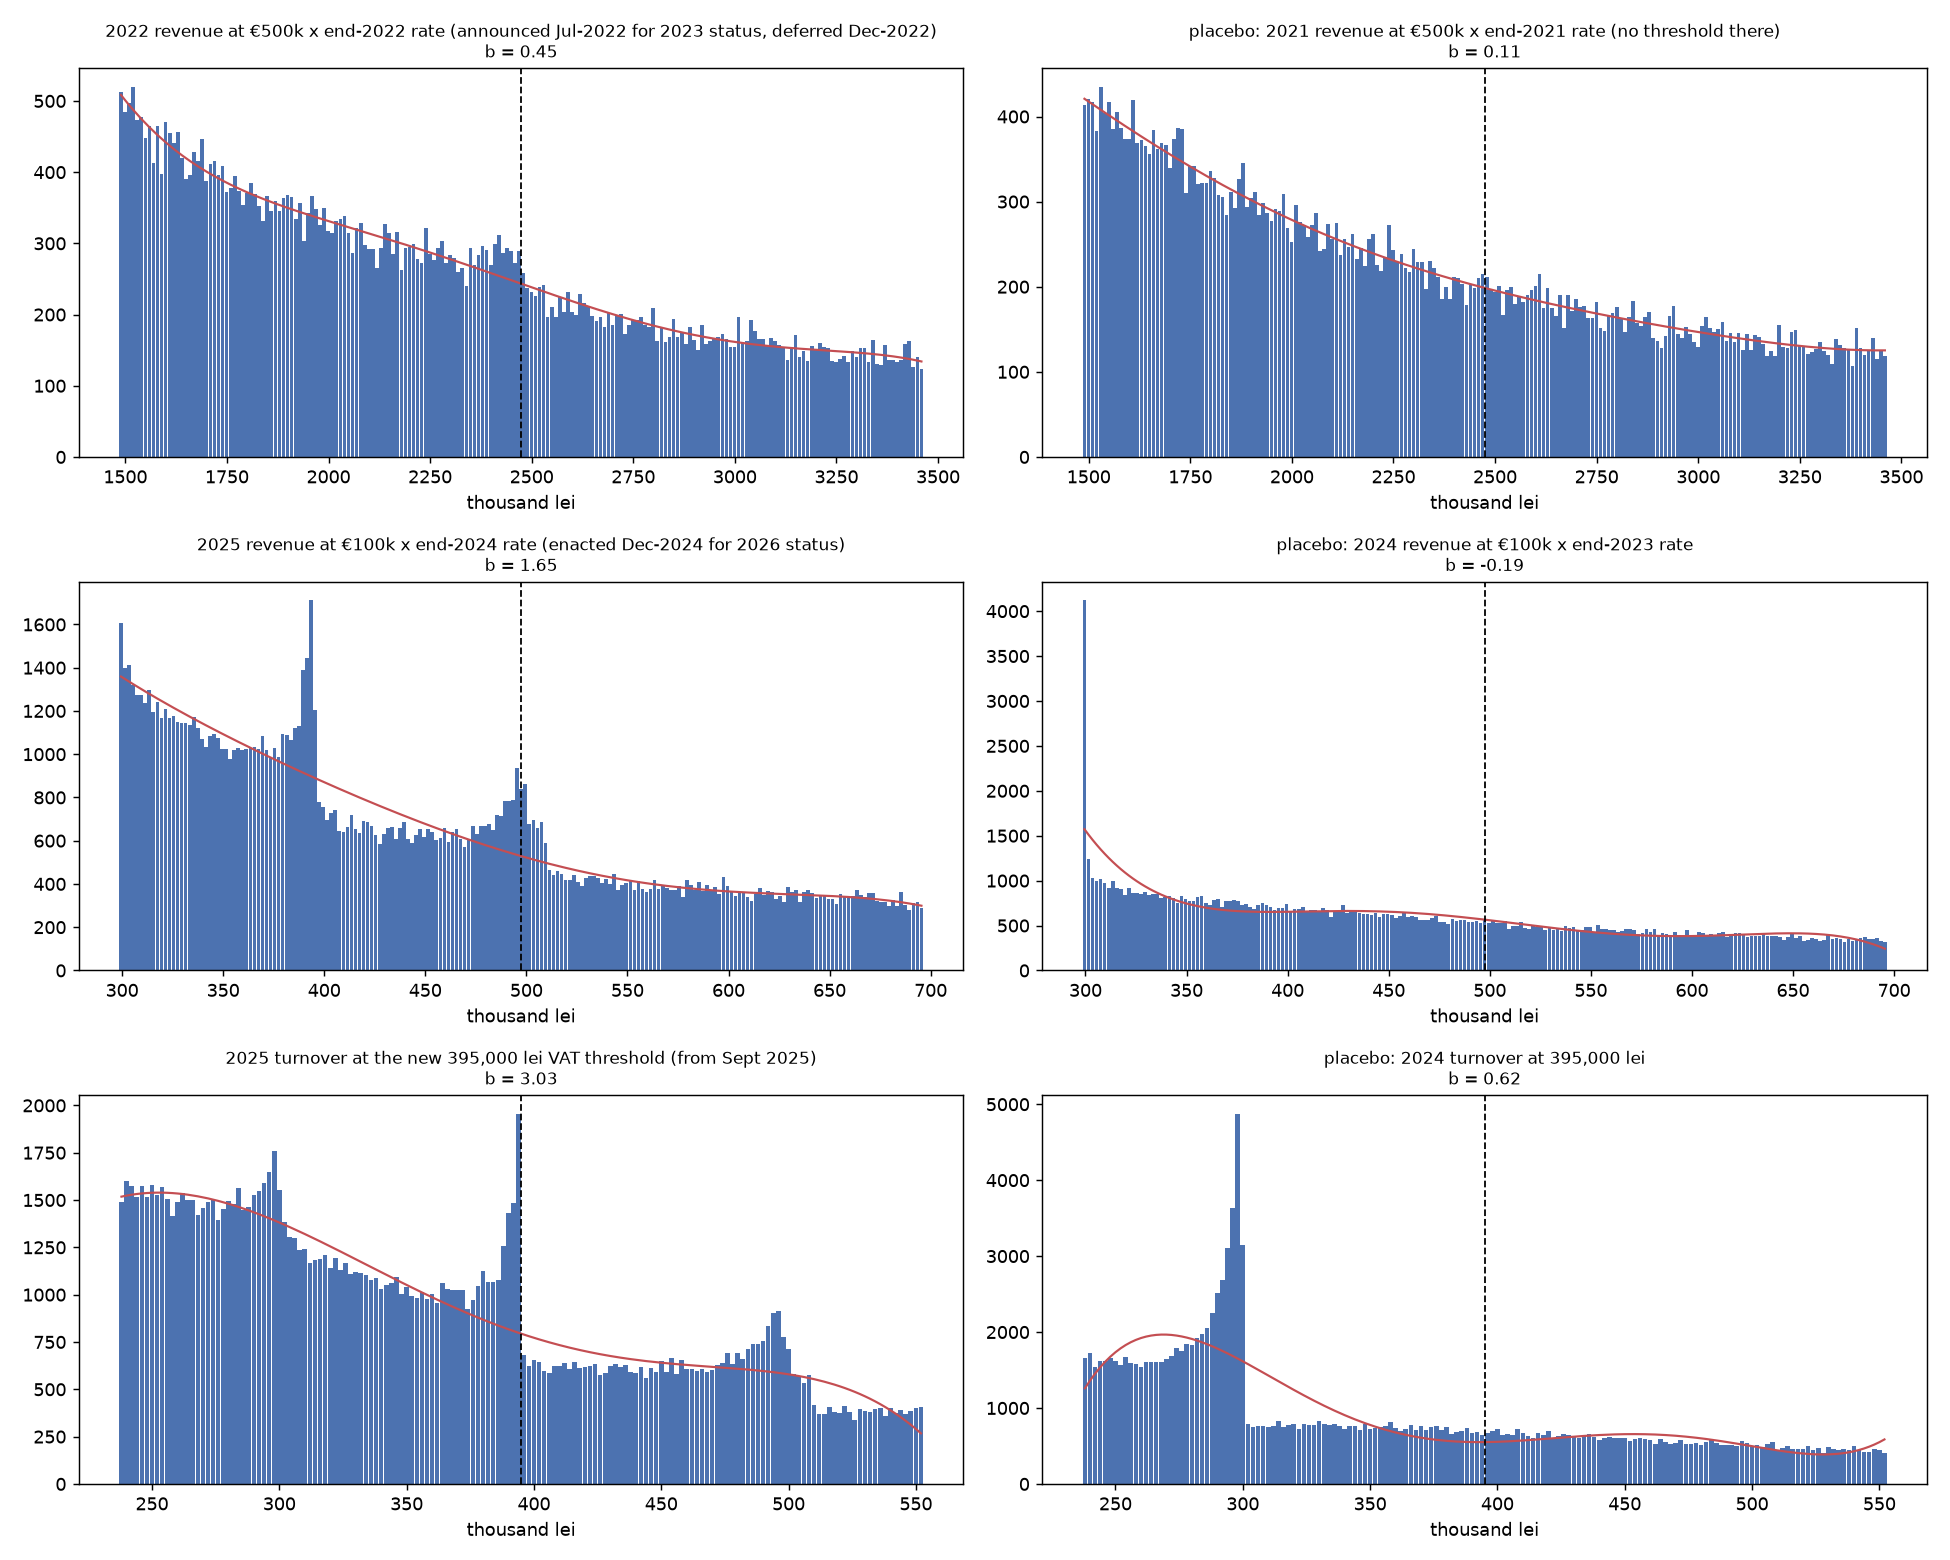
\includegraphics[width=\textwidth]{anticipation_checks.png}
\caption{Revenue around announced or enacted future ceilings and the new VAT threshold, with placebo years. Top: 2022 revenue at \euro{}500,000, announced in July 2022 for 2023 status and deferred in December 2022, with 2021 placebo. Middle: 2025 revenue at \euro{}100,000 at the end-2024 rate, enacted December 2024 for 2026 status, with 2024 placebo. Bottom: 2025 turnover at 395,000 lei with 2024 placebo. Polynomial counterfactuals for reference.}\label{fig:twonotch}
\end{figure}

\begin{figure}[!tbp]\centering
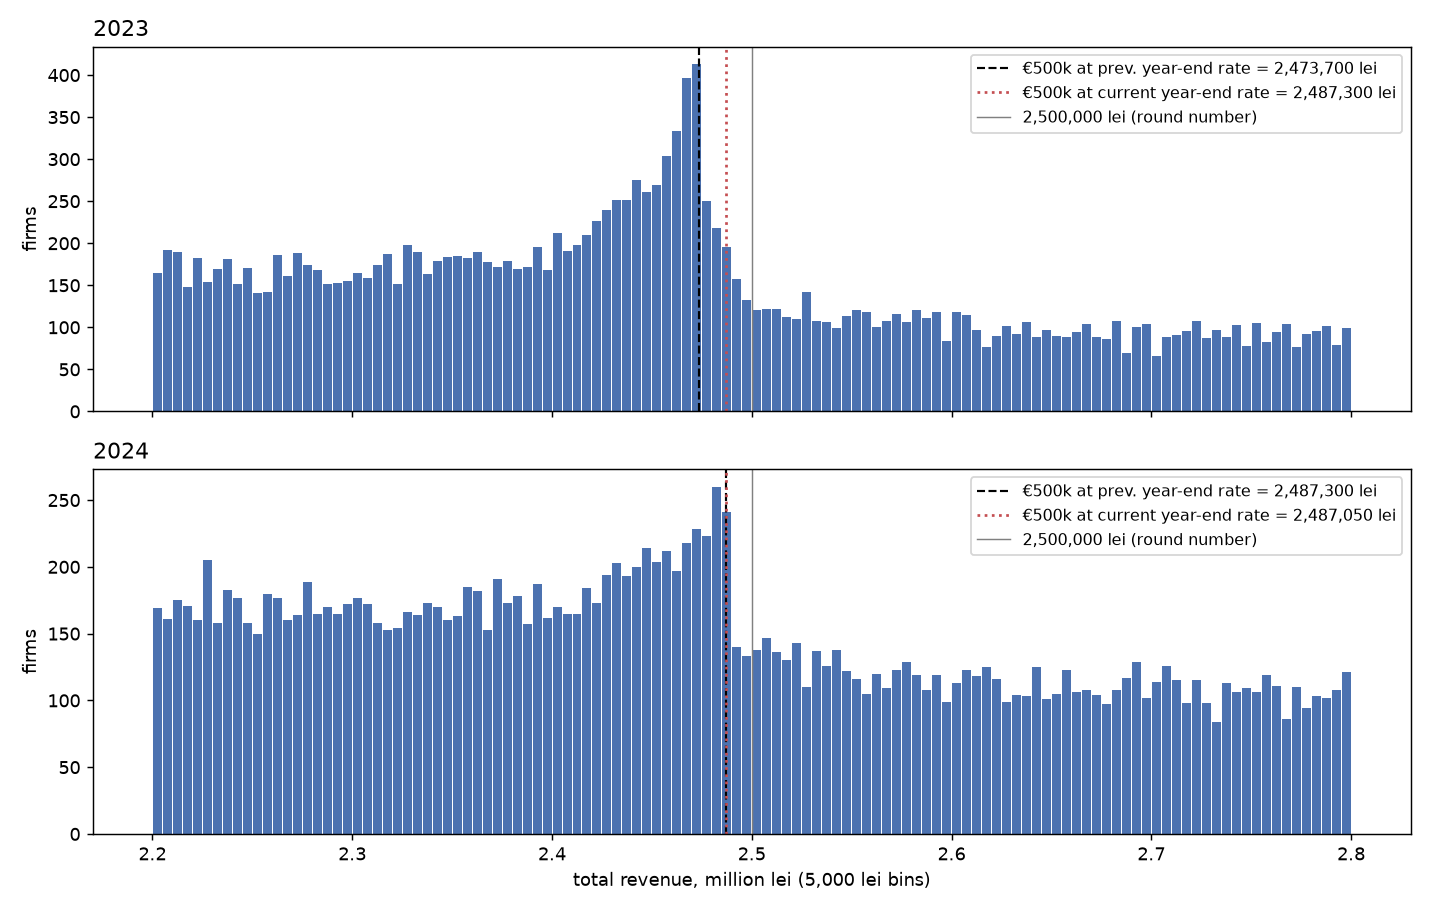
\includegraphics[width=0.85\textwidth]{lei_tracking_500k_2023_2024.png}
\caption{Total revenue in lei around \euro{}500,000, 2023 and 2024, 5,000-lei bins. The grey line marks 2,500,000 lei, the nearest round number.}\label{fig:lei500}
\end{figure}

\begin{figure}[!tbp]\centering
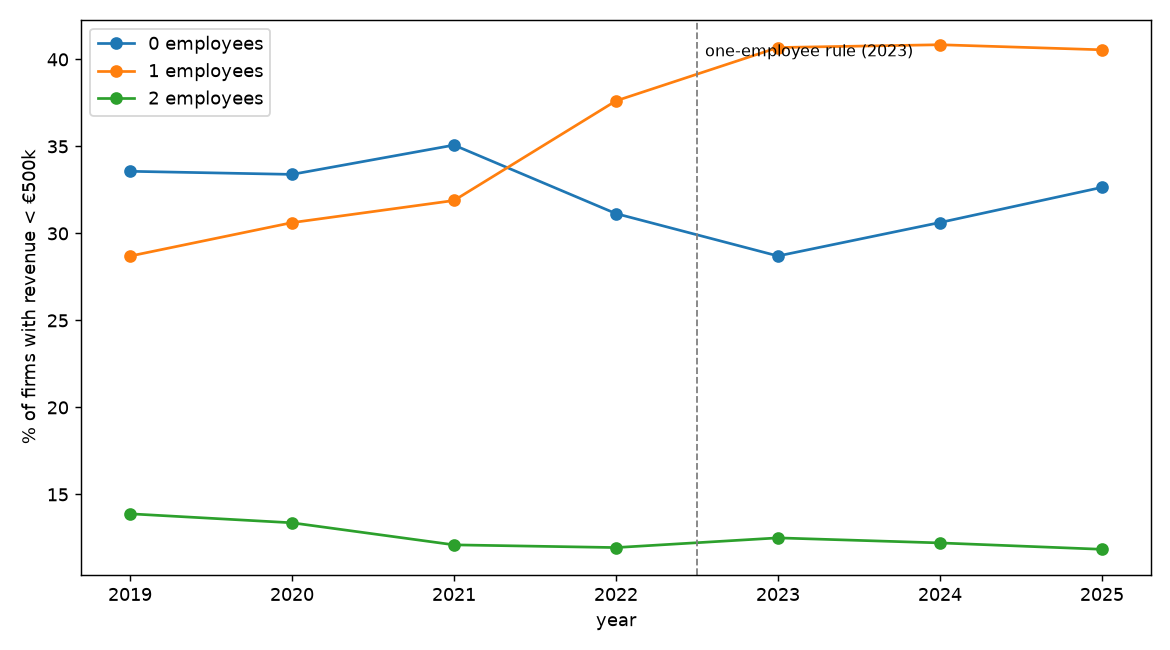
\includegraphics[width=0.8\textwidth]{employee_margin.png}
\caption{Share of firms with revenue below \euro{}500,000 reporting zero, one and two employees, 2019--2025.}\label{fig:emp}
\end{figure}
\FloatBarrier

\end{document}
